%  LaTeX support: latex@mdpi.com 
%  For support, please attach all files needed for compiling as well as the log file, and specify your operating system, LaTeX version, and LaTeX editor.

%=================================================================
\documentclass[jimaging,article,submit,pdftex,moreauthors]{Definitions/mdpi} 

% Figures live at repository root; this manuscript is compiled from draft/.
\graphicspath{{../}}
%\documentclass[preprints,article,submit,pdftex,moreauthors]{Definitions/mdpi} 
% For posting an early version of this manuscript as a preprint, you may use "preprints" as the journal. Changing "submit" to "accept" before posting will remove line numbers.

% Below journals will use APA reference format:
% admsci, aieduc, behavsci, businesses, econometrics, economies, education, ejihpe, famsci, games, humans, ijcs, ijfs, jintelligence, journalmedia, jrfm, jsam, languages, peacestud, psycholint, publications, tourismhosp, youth

% Below journals will use Chicago reference format:
% arts, genealogy, histories, humanities, laws, literature, religions, risks, socsci

%--------------------
% Class Options:
%--------------------
%----------
% journal
%----------
% Choose between the following MDPI journals:
% accountaudit, acoustics, actuators, addictions, adhesives, admsci, adolescents, aerobiology, aerospace, agriculture, agriengineering, agrochemicals, agronomy, ai, aichem, aieduc, aieng, aimater, aimed, aipa, air, aisens, algorithms, allergies, alloys, amh, analog, analytica, analytics, anatomia, anesthres, animals, antibiotics, antibodies, antioxidants, applbiosci, appliedchem, appliedmath, appliedphys, applmech, applmicrobiol, applnano, applsci, aquacj, architecture, arm, arthropoda, arts, asc, asi, astronautics, astronomy, atmosphere, atoms, audiolres, automation, axioms, bacteria, batteries, bdcc, behavsci, beverages, biochem, bioengineering, biologics, biology, biomass, biomechanics, biomed, biomedicines, biomedinformatics, biomimetics, biomolecules, biophysica, bioresourbioprod, biosensors, biosphere, biotech, birds, blockchains, bloods, blsf, brainsci, breath, buildings, businesses, cancers, carbon, cardio, cardiogenetics, cardiovascmed, catalysts, cells, ceramics, challenges, chemengineering, chemistry, chemosensors, chemproc, children, chips, cimb, civileng, cleantechnol, climate, clinbioenerg, clinpract, clockssleep, cmd, cmtr, coasts, coatings, colloids, colorants, commodities, complexities, complications, compounds, computation, computers, condensedmatter, conservation, constrmater, cosmetics, covid, crops, cryo, cryptography, crystals, csmf, ctn, culture, curroncol, cyber, dairy, data, ddc, dentistry, dermato, dermatopathology, designs, devices, dhi, diabetology, diagnostics, dietetics, digital, disabilities, diseases, diversity, dna, drones, dynamics, earth, ebj, ecm, ecologies, econometrics, economies, edm, education, eesp, ejihpe, electricity, electrochem, electronicmat, electronics, encyclopedia, endocrines, energies, eng, engproc, entomology, entropy, environments, environremediat, epidemiologia, epigenomes, esa, est, famsci, fermentation, fibers, fintech, fire, fishes, fluids, foods, forecasting, forensicsci, forests, fossstud, foundations, fractalfract, fuels, future, futureinternet, futurepharmacol, futurephys, futuretransp, galaxies, games, gases, gastroent, gastrointestdisord, gastronomy, gels, genealogy, genes, geographies, geohazards, geomatics, geometry, geosciences, geotechnics, geriatrics, germs, glacies, grasses, green, greenhealth, gucdd, hardware, hazardousmatters, healthcare, hearts, hemato, hematolrep, hep, heritage, higheredu, highthroughput, histories, horticulturae, hospitals, humanities, humans, hydrobiology, hydrogen, hydrology, hydropower, hygiene, idr, iic, ijcs, ijem, ijerph, ijfs, ijgi, ijmd, ijms, ijns, ijom, ijpb, ijt, ijtm, ijtpp, ime, immuno, informatics, information, infrastructures, inorganics, insects, instruments, inventions, iot, j, jaestheticmed, jal, jcdd, jcm, jcp, jcrm, jcs, jcto, jdad, jdb, jdream, jemr, jeta, jfb, jfmk, jgbg, jgg, jimaging, jintelligence, jlpea, jmahp, jmmp, jmms, jmp, jmse, jne, jnt, jof, joi, joitmc, joma, jop, joptm, jor, journalmedia, jox, jpbi, jphytomed, jpm, jrfm, jsam, jsan, jtaer, jvd, jzbg, kidneydial, kinasesphosphatases, knowledge, labmed, laboratories, lae, land, languages, laws, life, lights, limnolrev, lipidology, liquids, literature, livers, logics, logistics, lubricants, lymphatics, machines, macromol, magnetism, magnetochemistry, make, marinedrugs, materials, materproc, mathematics, mca, measurements, medicina, medicines, medsci, membranes, merits, metabolites, metals, meteorology, methane, metrics, metrology, micro, microarrays, microbiolres, microelectronics, micromachines, microorganisms, microplastics, microwave, minerals, mining, mmphys, modelling, molbank, molecules, mps, msf, mti, multimedia, muscles, nanoenergyadv, nanomanufacturing, nanomaterials, ncrna, ndt, network, neuroglia, neuroimaging, neurolint, neurosci, nitrogen, notspecified, nursrep, nutraceuticals, nutrients, obesities, occuphealth, oceans, ohbm, onco, optics, oral, organics, organoids, osteology, oxygen, pandemics, parasites, parasitologia, particles, pathogens, pathophysiology, peacestud, pediatrrep, pets, pharmaceuticals, pharmaceutics, pharmacoepidemiology, pharmacy, philosophies, photochem, photonics, phycology, physchem, physics, physiologia, plants, plasma, platforms, pollutants, polymers, polysaccharides, populations, poultry, powders, precipitation, precisoncol, preprints, proceedings, processes, prosthesis, proteomes, psf, psychiatryint, psychoactives, psycholint, publications, purification, quantumrep, quaternary, qubs, radiation, rdt, reactions, realestate, receptors, recycling, regeneration, religions, remotesensing, reports, reprodmed, resources, rheumato, risks, rjpm, robotics, rsee, ruminants, safety, sci, scipharm, sclerosis, seeds, sensors, separations, sexes, shi, signals, sinusitis, siuj, skins, smartcities, sna, societies, socsci, software, soilsystems, solar, solids, spectroscj, sports, standards, stats, std, stratsediment, stresses, surfaces, surgeries, suschem, sustainability, symmetry, synbio, systems, tae, targets, taxonomy, technologies, telecom, test, textiles, thalassrep, therapeutics, thermo, timespace, tomography, tourismhosp, toxics, toxins, tph, transplantology, transportation, traumacare, traumas, tri, tropicalmed, universe, urbansci, uro, vaccines, vehicles, venereology, vetsci, vibration, virtualworlds, viruses, vision, waste, water, welding, wem, wevj, wild, wind, women, world, youth, zoonoticdis

%---------
% article
%---------
% The default type of manuscript is "article", but can be replaced by: 
% abstract, addendum, article, benchmark, book, bookreview, briefcommunication, briefreport, casereport, changes, clinicopathologicalchallenge, comment, commentary, communication, conceptpaper, conferenceproceedings, correction, conferencereport, creative, datadescriptor, discussion, entry, expressionofconcern, extendedabstract, editorial, essay, erratum, fieldguide, hypothesis, interestingimages, letter, meetingreport, monograph, newbookreceived, obituary, opinion, proceedingpaper, projectreport, reply, retraction, review, perspective, protocol, shortnote, studyprotocol, supfile, systematicreview, technicalnote, viewpoint, guidelines, registeredreport, tutorial,  giantsinurology, urologyaroundtheworld
% supfile = supplementary materials

%----------
% submit
%----------
% The class option "submit" will be changed to "accept" by the Editorial Office when the paper is accepted. This will only make changes to the frontpage (e.g., the logo of the journal will get visible), the headings, and the copyright information. Also, line numbering will be removed. Journal info and pagination for accepted papers will also be assigned by the Editorial Office.

%------------------
% moreauthors
%------------------
% If there is only one author the class option oneauthor should be used. Otherwise use the class option moreauthors.

%---------
% pdftex
%---------
% The option pdftex is for use with pdfLaTeX. Remove "pdftex" for (1) compiling with LaTeX & dvi2pdf (if eps figures are used) or for (2) compiling with XeLaTeX.

%=================================================================
% MDPI internal commands - do not modify
\firstpage{1} 
\makeatletter 
\setcounter{page}{\@firstpage} 
\makeatother
\pubvolume{1}
\issuenum{1}
\articlenumber{0}
\pubyear{2026}
\copyrightyear{2026}
%\externaleditor{Firstname Lastname} % More than 1 editor, please add `` and '' before the last editor name
\datereceived{} 
\daterevised{} % Comment out if no revised date
\dateaccepted{} 
\datepublished{} 
%\datecorrected{} % For corrected papers: "Corrected: XXX" date in the original paper.
%\dateretracted{} % For retracted papers: "Retracted: XXX" date in the original paper.
%\doinum{} % Used for some special journals, like molbank
%\pdfoutput=1 % Uncommented for upload to arXiv.org
%\CorrStatement{yes}  % For updates
%\longauthorlist{yes} % For many authors that exceed the left citation part
%\IsAssociation{yes} % For association journals

%=================================================================
% Add packages and commands here. The following packages are loaded in our class file: fontenc, inputenc, calc, indentfirst, fancyhdr, graphicx, epstopdf, lastpage, ifthen, float, amsmath, amssymb, lineno, setspace, enumitem, mathpazo, booktabs, titlesec, etoolbox, tabto, xcolor, colortbl, soul, multirow, microtype, tikz, totcount, changepage, attrib, upgreek, array, tabularx, pbox, ragged2e, tocloft, marginnote, marginfix, enotez, amsthm, natbib, hyperref, cleveref, scrextend, url, geometry, newfloat, caption, draftwatermark, seqsplit
% cleveref: load \crefname definitions after \begin{document}

\usepackage{algorithm}
\usepackage{algpseudocode}

%=================================================================
% Please use the following mathematics environments: Theorem, Lemma, Corollary, Proposition, Characterization, Property, Problem, Example, ExamplesandDefinitions, Hypothesis, Remark, Definition, Notation, Assumption
%% For proofs, please use the proof environment (the amsthm package is loaded by the MDPI class).

%=================================================================
% Full title of the paper (Capitalized)
\Title{HypEReg-TransMorph: A Hyperelastic-Regularized Transformer\\ Framework for Folding-Suppressed Deformable Brain MRI Registration}

% Author Orchid ID: enter ID or remove command
\newcommand{\orcidauthorA}{0000-0000-0000-000X} % TODO: replace with Mohan Xu's ORCID; add \orcidA{} behind the author's name
%\newcommand{\orcidauthorB}{0000-0000-0000-000X} % Add \orcidB{} behind the author's name

% Authors, for the paper (add full first names)
\Author{Shiyi Xu $^{1}$ and Mohan Xu $^{2,*}$\orcidA{}}

%\longauthorlist{yes}

% MDPI internal command: Authors, for metadata in PDF
\AuthorNames{Shiyi Xu and Mohan Xu}

%\longauthorlist{yes}

% Affiliations / Addresses (Add [1] after \address if there is only one affiliation.)
\address{%
$^{1}$ \quad Capital Medical University, Beijing 100069, China; xsy4831@mail.ccmu.edu.cn\\
$^{2}$ \quad School of Physics, Peking University, Beijing 100871, China; 2200011601@stu.pku.edu.cn}

% Contact information of the corresponding author
\corres{Correspondence: Mohan Xu; 2200011601@stu.pku.edu.cn}

% Current address and/or shared authorship
%\firstnote{Current address: Affiliation.}  
% Current address should not be the same as any items in the Affiliation section.

%\secondnote{These authors contributed equally to this work.}
% The commands \thirdnote{} till \eighthnote{} are available for further notes.

%\simplesumm{} % Simple summary

%\conference{} % An extended version of a conference paper

% Abstract (Do not insert blank lines, i.e. \\) 
\abstract{Background: Deformable brain MRI registration requires accurate alignment and geometrically plausible deformation fields. Methods: Hyperelastic-energy regularization (HypEReg) is integrated into a TransMorph-style dense registration backbone to penalize implausible local volume change and folding. Evaluation is performed on a held-out IXI atlas-to-subject test protocol using grouped anatomical labels and paired inferential analysis. Results: HypEReg-TransMorph maintains overlap performance comparable to strong Transformer baselines while substantially improving deformation regularity and folding suppression. Conclusions: These findings support Jacobian-aware regularization as a practical strategy for improving deformation plausibility in Transformer-based neuroimaging registration workflows, with direct relevance to downstream clinical applications such as Jacobian-based morphometric biomarkers, atlas-based segmentation for treatment planning, and longitudinal disease monitoring.}

% Keywords
\keyword{medical image registration; deformable registration; transformer; hyperelastic-energy regularization; HypEReg-TransMorph; folding suppression; Jacobian regularization; Jacobian determinant; brain MRI}

% The fields PACS, MSC, and JEL may be left empty or commented out if not applicable
%\PACS{J0101}
%\MSC{}
%\JEL{}

%%%%%%%%%%%%%%%%%%%%%%%%%%%%%%%%%%%%%%%%%%
% Only for the journal Diversity
%\LSID{\url{http://}}

%%%%%%%%%%%%%%%%%%%%%%%%%%%%%%%%%%%%%%%%%%
% Only for the journal Applied Sciences
%\featuredapplication{Authors are encouraged to provide a concise description of the specific application or a potential application of the work. This section is not mandatory.}
%%%%%%%%%%%%%%%%%%%%%%%%%%%%%%%%%%%%%%%%%%

%%%%%%%%%%%%%%%%%%%%%%%%%%%%%%%%%%%%%%%%%%
% Only for the journal Data
%\dataset{DOI number or link to the deposited data set if the data set is published separately. If the data set shall be published as a supplement to this paper, this field will be filled by the journal editors. In this case, please submit the data set as a supplement.}
%\datasetlicense{License under which the data set is made available (CC0, CC-BY, CC-BY-SA, CC-BY-NC, etc.)}

%%%%%%%%%%%%%%%%%%%%%%%%%%%%%%%%%%%%%%%%%%
% Only for the journal BioTech, Fishes, Neuroimaging and Toxins
%\keycontribution{The breakthroughs or highlights of the manuscript. Authors can write one or two sentences to describe the most important part of the paper.}

%%%%%%%%%%%%%%%%%%%%%%%%%%%%%%%%%%%%%%%%%%
% Only for the journal Encyclopedia
%\encyclopediadef{For entry manuscripts only: please provide a brief overview of the entry title instead of an abstract.}

%%%%%%%%%%%%%%%%%%%%%%%%%%%%%%%%%%%%%%%%%%
% Different journals have different requirements. Please check the specific journal guidelines in the "Instructions for Authors" on the journal's official website.
%\addhighlights{yes}
%\renewcommand{\addhighlights}{%
%
%\noindent The goal is to increase the discoverability and readability of the article via search engines and other scholars. Highlights should not be a copy of the abstract, but a simple text allowing the reader to quickly and simplified find out what the article is about and what can be cited from it. Each of these parts should be devoted up to 2~bullet points.\vspace{3pt}\\
%\textbf{What are the main findings?}
% \begin{itemize}[labelsep=2.5mm,topsep=-3pt]
% \item First bullet.
% \item Second bullet.
% \end{itemize}\vspace{3pt}
%\textbf{What are the implications of the main findings?}
% \begin{itemize}[labelsep=2.5mm,topsep=-3pt]
% \item First bullet.
% \item Second bullet.
% \end{itemize}
%}

%%%%%%%%%%%%%%%%%%%%%%%%%%%%%%%%%%%%%%%%%%
\begin{document}

%%%%%%%%%%%%%%%%%%%%%%%%%%%%%%%%%%%%%%%%%%
\section{Introduction}

Deformable registration is a central component of computational neuroimaging pipelines, including atlas propagation, longitudinal analysis, and voxel-wise morphometry. In recent years, learning-based methods have significantly reduced inference time compared with classical iterative optimization \cite{balakrishnan2019voxelmorph,kim2021cyclemorph}. However, high overlap metrics alone are not sufficient when deformation fields contain local foldings or implausible volume changes.

Transformer-based registration improves long-range contextual modeling and has shown strong performance on 3D MRI tasks \cite{chen2022transmorph}. Nevertheless, unconstrained displacement prediction may still produce non-diffeomorphic deformations, which can invalidate downstream Jacobian-based analysis. To address this, we adapt a Jacobian-aware regularization scheme derived from hyperelastic principles \cite{burger2013hyperelastic} to a TransMorph backbone and explicitly optimize deformation plausibility. We refer to this regularizer as HypEReg, with the explicit caveat that we use a deep-learning--friendly two-term subset (volume distortion and anti-folding) rather than the full polyconvex hyperelastic energy.

\noindent\textbf{Clinical motivation.} The need for diffeomorphic, fold-free deformations is not a purely mathematical concern: in clinical neuroimaging, the Jacobian determinant of the registration field is itself the quantity reported in tensor-based morphometry (TBM) and longitudinal atrophy/expansion studies for Alzheimer's disease, mild cognitive impairment, multiple sclerosis, normal-pressure hydrocephalus, and post-surgical follow-up of brain tumors and epilepsy resections. When local foldings (\(\det J_\phi \le 0\)) appear in the deformation field, the corresponding voxels report negative or undefined volume change, biasing voxel-wise statistical maps and inflating false-positive clusters at the boundaries of ventricles, cortex and deep gray nuclei---precisely the structures of greatest clinical interest. Equivalently, in atlas-based segmentation (FreeSurfer-style and SPM-style pipelines used for radiotherapy planning, deep brain stimulation targeting, and surgical navigation), label propagation through a folded warp can produce anatomically inconsistent boundaries that must be manually corrected. Constraining the registration field to be near-diffeomorphic at training time therefore directly reduces downstream clinical post-processing burden and improves the trustworthiness of derived biomarkers, while preserving the inference-time speed of feed-forward learned models that is essential for clinical throughput.

The contributions of this study are positioned, deliberately, as engineering-level rather than theoretical:
\begin{itemize}
\item An empirical instantiation of a Jacobian-aware regularizer derived from hyperelastic principles inside a Transformer-based dense-displacement registration framework (HypEReg-TransMorph), explicitly distinct from prior CNN/U-Net implementations of related volume-change and anti-folding penalties \cite{mok2020fast,hering2021lung} and from concurrent linear-elastic and hyperelastic regularizers in deep registration \cite{zou2023conformal,elasticmorph2025};
\item A unified IXI atlas-to-subject benchmark that quantifies the trade-off between grouped-VOI overlap and deformation regularity across deep-learning baselines and a classical SyN reference, including paired Wilcoxon/BH-FDR inferential analysis;
\item A reproducibility package (code, configurations, per-case metric exports, and figure scripts) released openly so that the regularization design and evaluation protocol can be reused as a drop-in component on TransMorph-style backbones.
\end{itemize}

\section{Related Work}

\subsection{Classical and Diffeomorphic Registration}
Classical registration frameworks such as SyN and related diffeomorphic formulations remain strong references for deformation plausibility, because they explicitly constrain transformation smoothness and invertibility during optimization \cite{avants2008ants,rueckert1999nonrigid,ashburner1999morphometry}. These methods often provide robust topology behavior but at substantially higher computational cost than feed-forward learned models.

\subsection{Learning-Based Dense Registration}
Learning-based methods, represented by VoxelMorph and descendants, provide fast inference with strong overlap accuracy \cite{balakrishnan2019voxelmorph}. Subsequent CNN and hybrid variants (e.g., CycleMorph and MIDIR) improve representational capacity \cite{kim2021cyclemorph}, while probabilistic diffeomorphic variants aim to improve deformation stability \cite{dalca2019probreg}. Even so, unconstrained dense displacement prediction can still produce locally implausible Jacobian behavior.

\subsection{Transformer-Based Registration}
Transformer backbones improve long-range context modeling in volumetric registration and have become competitive baselines \cite{chen2022transmorph,liu2021swin}. In this manuscript, CoTr, nnFormer, and PVT are treated as adapted Transformer-family backbones used in the same IXI evaluation workflow \cite{xie2021cotr,zhou2023nnformer,wang2021pvt}. For each backbone, the registration adapter concatenates moving/fixed images as a two-channel input and uses the repository flow-prediction decoder head to output \((I_w,\phi)\); all three adapters are evaluated under the same atlas-to-subject protocol. The objective here is not to propose a new Transformer architecture, but to evaluate training-time regularization on a TransMorph-style dense-flow network.

\subsection{Hyperelastic and Jacobian-Based Regularization}
Jacobian-aware and hyperelastic penalties provide direct control of local volume change and folding behavior \cite{burger2013hyperelastic}. These terms complement smoothness regularizers by explicitly penalizing singular or near-singular deformation regions, which is important for downstream morphometric interpretation. The original Burger--Modersitzki--Ruthotto formulation combines length, surface (cofactor) and volume terms inside a polyconvex energy and proves existence of minimizers in a discretize-then-optimize variational setting; in our deep-learning setting, we use only a Jacobian-aware subset of this family, and we discuss this divergence explicitly in Section~\ref{sec:loss}.

\subsection{Volume-Preserving and Anti-Folding Regularization in Deep Registration}
Several recent learning-based works place Jacobian-aware penalties directly into the training objective of deep registration networks. \citet{mok2020fast} introduce a selective Jacobian-determinant penalty that activates on $\det J\le 0$ regions inside a fast symmetric diffeomorphic CNN; this term is conceptually the immediate antecedent of our anti-folding hinge $\mathcal{L}_{\mathrm{fold}}$. \citet{hering2021lung} place a volume-change penalty together with a curvature regularizer inside a CNN-based lung-CT registration pipeline, demonstrating that BMR-style volume control can be incorporated into deep registration loss functions. \citet{zou2023conformal} adopt a non-linear conformal-invariant hyperelastic energy in a deep registration framework on lung CT, providing the closest precedent for hyperelastic-style regularization in learned registration. The recent \emph{ElasticMorph} framework \cite{elasticmorph2025} plugs a second-order Navier--Cauchy linear-elastic regularizer into TransMorph and VoxelMorph backbones and reports overlap improvements with reduced folding artifacts on IXI/LPBA40 brain registration. Compared with these works, the contribution of HypEReg-TransMorph is restricted in scope: we do not propose a new architecture or a new theoretical regularizer; instead we report a practical configuration that combines a simplified rational volume-change term with an explicit anti-folding hinge inside a TransMorph backbone, and we evaluate the resulting trade-off under the IXI atlas-to-subject protocol with paired inferential statistics. We discuss the precise differences in formulation in Section~\ref{sec:loss} and the experimental positioning relative to ElasticMorph in Section~5.

%%%%%%%%%%%%%%%%%%%%%%%%%%%%%%%%%%%%%%%%%%
\section{Materials and Methods}

\subsection{Dataset and Preprocessing}
Experiments use the IXI brain MRI dataset \cite{ixidataset} under an atlas-to-subject registration protocol with a 403/58/115 train/validation/test split. All reported metrics are computed on the 115 held-out test subjects. This study uses the T1-weighted preprocessed IXI package commonly adopted by TransMorph-style studies \cite{chen2022transmorph,kim2021cyclemorph}, where preprocessing includes skull stripping, affine alignment, and subcortical segmentation generation in the published preprocessing workflow. Volumes are represented in a common template space and cropped/resampled to \(160 \times 192 \times 224\). A shared fixed atlas image-label pair is used for all methods. Intensity images are warped with trilinear interpolation and label maps with nearest-neighbor interpolation in evaluation/training utilities.


\begin{table}[H]
\caption{Dataset, preprocessing, and protocol summary.\label{tab1}}
\begin{tabularx}{\textwidth}{lX}
\toprule
\textbf{Item} & \textbf{Configuration} \\
\midrule
Dataset source & IXI project dataset \cite{ixidataset} and preprocessed IXI package used in TransMorph-style workflows \\
License & IXI public dataset terms (CC BY-SA 3.0 at IXI portal); preprocessed release follows its repository terms \\
Volumes and split & 576 preprocessed subjects + atlas; 403 / 58 / 115 (train / validation / test) \\
Modality and task & T1-weighted structural MRI; atlas-to-subject deformable registration \\
Input shape & \(160 \times 192 \times 224\) after preprocessing/cropping \\
Preprocessing summary & Public preprocessed IXI workflow (including skull stripping, affine alignment, and segmentation preprocessing) with template-space normalization; same pipeline used across all compared methods \\
Labels and grouped VOIs & Segmentation labels are aggregated into 17 bilateral/related VOI groups for grouped Dice analysis \\
Atlas definition & Fixed atlas image/label pair; same atlas used for all methods \\
Interpolation & Intensity: trilinear warping; labels: nearest-neighbor warping \\
Metric spacing & Surface metrics (HD95/ASSD/NSD) use spacing-aware distance transforms in the evaluation metrics implementation \\
Compared families & TransMorph-family baselines, CNN/hybrid baselines, and classical SyN \\
\bottomrule
\end{tabularx}
\end{table}

\subsection{Baseline Model}
The base architecture is TransMorph, a Transformer-based dense deformable registration network with a Swin-style encoder and decoder-to-flow prediction head \cite{chen2022transmorph,liu2021swin}. We compare HypEReg-TransMorph against deep-learning and classical baselines under identical preprocessing and evaluation scripts:
\begin{itemize}
\item Transformer family: TransMorph~\cite{chen2022transmorph}, TransMorphBayes (Bayesian variant from~\cite{chen2022transmorph}), CoTr~\cite{xie2021cotr}, nnFormer~\cite{zhou2023nnformer}, PVT~\cite{wang2021pvt};
\item CNN / hybrid baselines: VoxelMorph-1~\cite{balakrishnan2019voxelmorph}, CycleMorph~\cite{kim2021cyclemorph}, MIDIR;
\item Classical baseline: SyN (ANTs)~\cite{avants2008ants}.
\end{itemize}
Checkpoint and version identifiers are documented in the repository evaluation configuration and the supplementary checkpoint manifest.
Published baseline checkpoints were obtained from official repositories. For checkpoints where exact upstream training splits cannot be independently verified from model cards/releases, this is explicitly treated as a fairness limitation and documented in the reproducibility notes.

\subsection{Proposed HypEReg-TransMorph Framework}
HypEReg-TransMorph augments the TransMorph baseline with explicit hyperelastic regularization to constrain unrealistic local distortion. The operating-point regularizer targets two complementary aspects of deformation quality: volume-change moderation and anti-folding behavior near singular Jacobian regions. A length-change term is retained in the general mathematical formulation but its coefficient is set to zero in the final operating point because \(\mathcal{L}_{\mathrm{grad}}\) already constrains displacement smoothness and length-change behavior.

Figure~\ref{fig1} summarizes the training architecture. The moving image \(I_m\) and fixed image \(I_f\) are concatenated and passed through a TransMorph-style backbone with a Transformer encoder and CNN decoder, producing a dense displacement field \(u\). The deformation is parameterized as \(\phi=\mathrm{Id}+u\), and a spatial transformer module warps \(I_m\) to obtain \(I_w\). Three losses are then aggregated into a single objective: similarity \(\mathcal{L}_{\mathrm{sim}}(I_w,I_f)\), smoothness \(\mathcal{L}_{\mathrm{grad}}(u)\), and hyperelastic regularization \(\mathcal{L}_{\mathrm{HypEReg}}(u)\). The training-time HypEReg loss computation path evaluates \(J_\phi=I+\nabla u\) and \(\det J_\phi\), from which length, volume, and folding penalties are formed; in the final operating point, \(\alpha=0\), \(\beta=0.02\), and \(\gamma=20\), so the active HypEReg supervision is the volume + anti-folding subset. The network is trained with directional symmetry updates \((x\rightarrow y)\) and \((y\rightarrow x)\), and each direction performs its own forward/backward/optimizer step:
\begin{linenomath}
\begin{equation}
\mathcal{L}_{\mathrm{total}}
=
\mathcal{L}_{\mathrm{sim}}(I_w,I_f)
+
\lambda_{\mathrm{grad}}\mathcal{L}_{\mathrm{grad}}(u)
+
\lambda_{\mathrm{HypEReg}}\mathcal{L}_{\mathrm{HypEReg}}(u).
\end{equation}
\end{linenomath}

\begin{figure}[t]
\centering
\IfFileExists{HER.png}{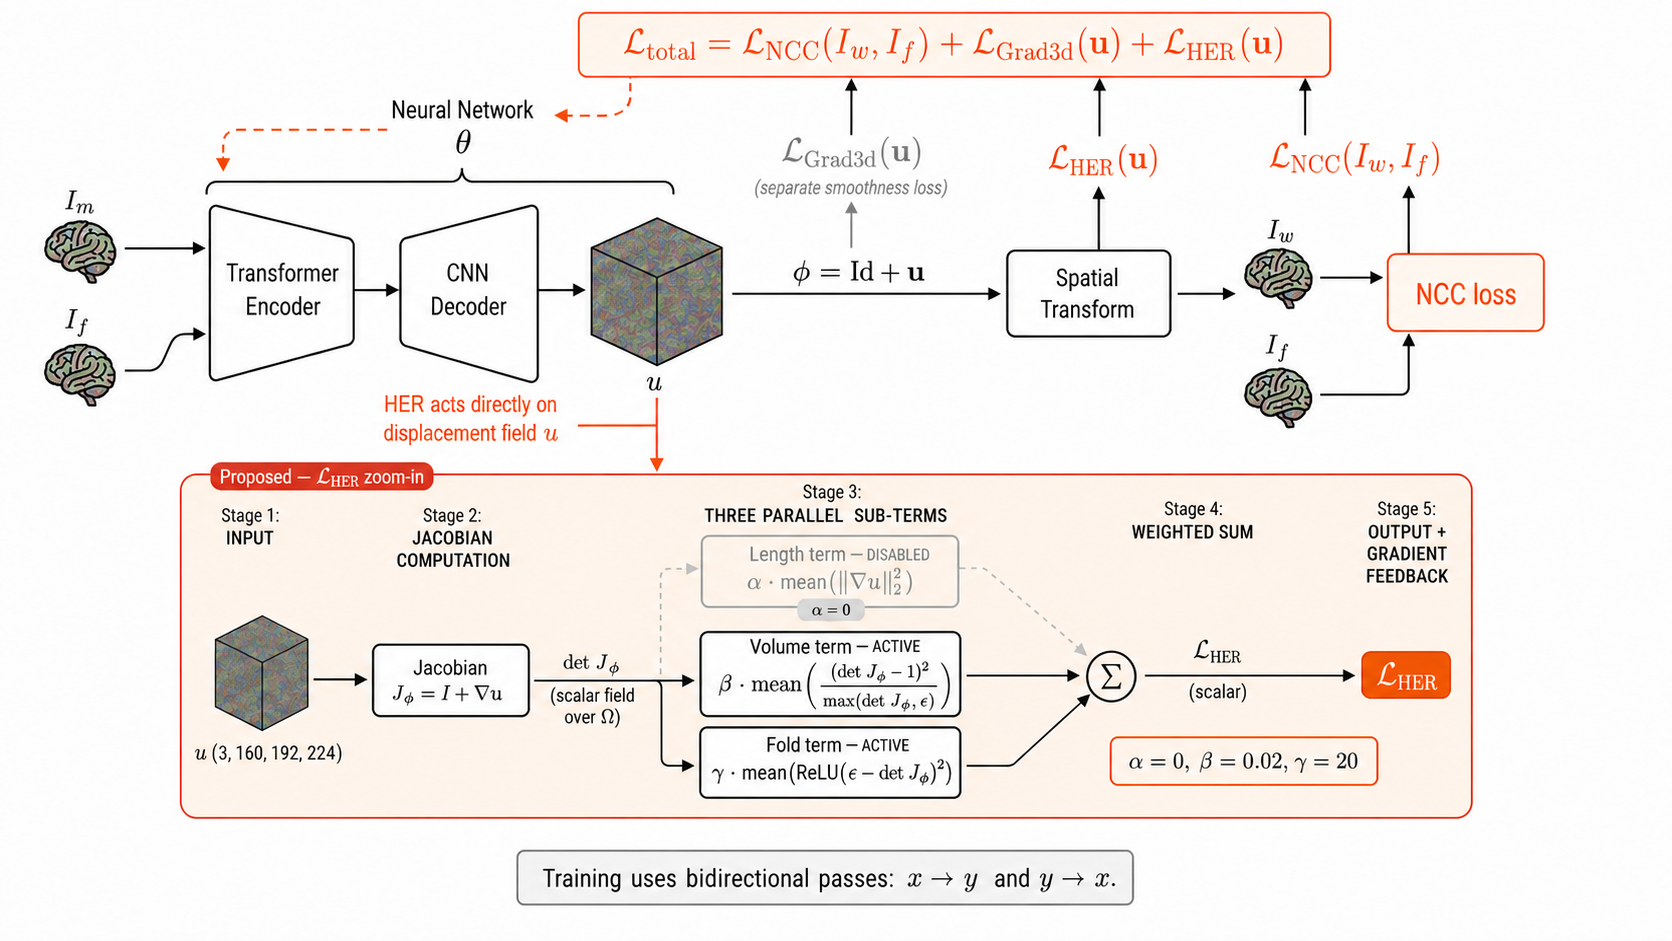
\includegraphics[width=0.96\textwidth]{HER.png}}{\IfFileExists{../HER.png}{
\includegraphics[width=0.96\textwidth]{../HER.png}}{\IfFileExists{../figures/HER.png}{
\includegraphics[width=0.96\textwidth]{../figures/HER.png}}{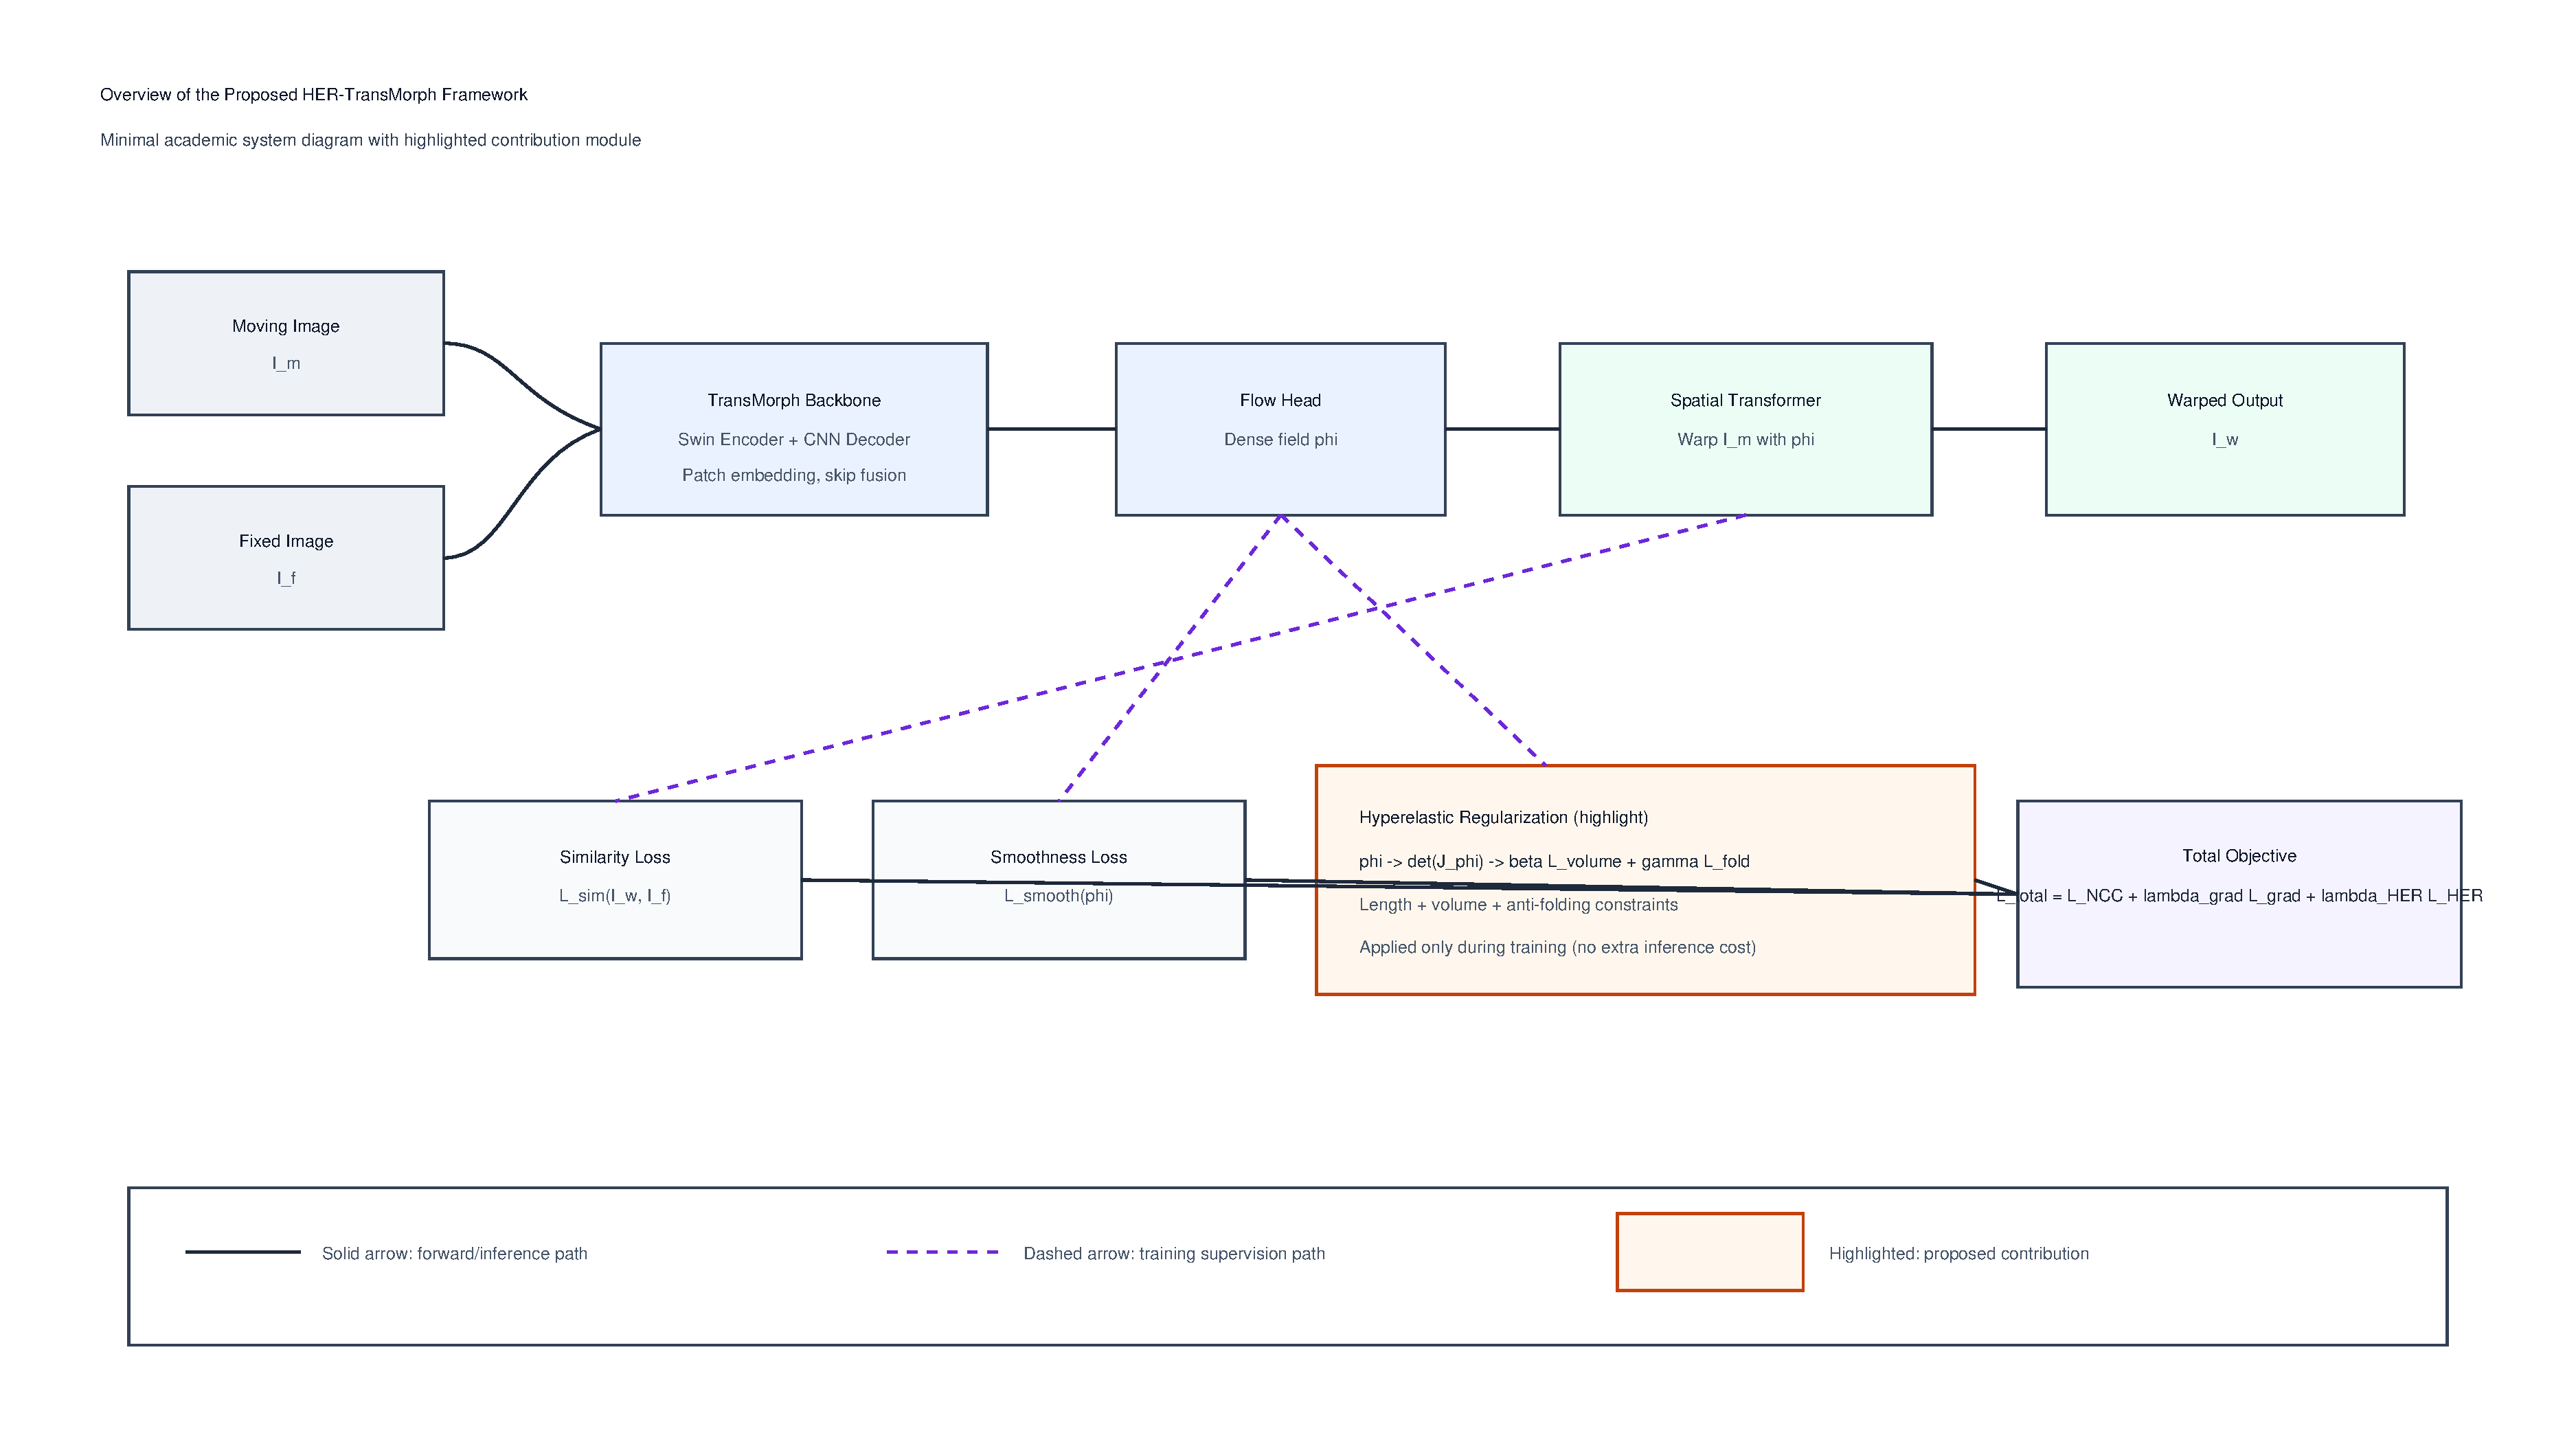
\includegraphics[width=0.96\textwidth]{figures/fig1_framework_figma.pdf}}}}
\caption{Architecture and training objective of the proposed HypEReg-TransMorph framework. The moving image (\(I_m\)) and fixed image (\(I_f\)) are concatenated and passed through a TransMorph-based registration network with a Transformer encoder and CNN decoder to predict a dense 3D displacement field (\(u\)). The deformation transform is defined as \(\phi=\mathrm{Id}+u\), and a spatial transformer warps the moving image to generate the warped image (\(I_w\)). During training, three complementary terms are optimized: similarity loss \(\mathcal{L}_{\mathrm{sim}}(I_w,I_f)\), smoothness \(\lambda_{\mathrm{grad}}\mathcal{L}_{\mathrm{grad}}(u)\), and hyperelastic regularization \(\lambda_{\mathrm{HypEReg}}\mathcal{L}_{\mathrm{HypEReg}}(u)\), with \(\mathcal{L}_{\mathrm{sim}}=-\overline{\mathrm{LCC}^{\,2}}(I_w,I_f)\). The total objective is \(\mathcal{L}=\mathcal{L}_{\mathrm{sim}}+\lambda_{\mathrm{grad}}\mathcal{L}_{\mathrm{grad}}+\lambda_{\mathrm{HypEReg}}\mathcal{L}_{\mathrm{HypEReg}}\). The HypEReg zoom-in panel details computation of \(\mathcal{L}_{\mathrm{HypEReg}}\): \(u\rightarrow J_\phi=I+\nabla u\rightarrow \det J_\phi\rightarrow\) length/volume/folding sub-terms. In the final operating point, the length term is disabled (\(\alpha=0\)), while volume and folding terms remain active (\(\beta=0.02\), \(\gamma=20\)). Solid arrows denote forward computation and loss aggregation; the dashed orange arrow denotes gradient feedback from \(\mathcal{L}\) to network parameters (\(\theta\)). Training uses bidirectional passes (\(x\rightarrow y\), \(y\rightarrow x\)). In the schematic graphic, the regularization branch is labeled with subscript \(\mathrm{HER}\) as a compact shorthand for the HypEReg term \(\mathcal{L}_{\mathrm{HypEReg}}\) used throughout the manuscript.\label{fig1}}
\end{figure}

\subsection{Loss Function}
\label{sec:loss}
The deformation is defined as \(\phi(x)=x+u(x)\), where \(u:\Omega\rightarrow\mathbb{R}^3\) is the dense displacement field. The unified training objective is
\begin{linenomath}
\begin{equation}
\mathcal{L}_{\mathrm{total}}
=
\mathcal{L}_{\mathrm{sim}}
+
\lambda_{\mathrm{grad}}\mathcal{L}_{\mathrm{grad}}
+
\lambda_{\mathrm{HypEReg}}\left(
\alpha \mathcal{L}_{\mathrm{length}} + \beta \mathcal{L}_{\mathrm{volume}} + \gamma \mathcal{L}_{\mathrm{fold}}
\right).
\end{equation}
\end{linenomath}
Here, \(\mathcal{L}_{\mathrm{sim}}=-\overline{\mathrm{LCC}^{\,2}}(I_w,I_f)\) is the negative mean squared local correlation between the warped and fixed images, evaluated with a \(9^3\) sliding window as in the VoxelMorph reference implementation \cite{balakrishnan2019voxelmorph} (this is the form commonly referred to as ``local NCC'' in the deep registration literature). The smoothness term in the unified objective is the squared first-order finite-difference penalty
\begin{linenomath}
\begin{equation}
\mathcal{L}_{\mathrm{grad}}(u)
=
\tfrac{1}{3}\Big(\overline{|\partial_x u|^{\,2}}+\overline{|\partial_y u|^{\,2}}+\overline{|\partial_z u|^{\,2}}\Big),
\end{equation}
\end{linenomath}
where the overline denotes voxel-wise and channel-wise mean and \(\partial_d\) is forward finite difference along axis \(d\); this is the standard squared-L2 gradient penalty used in the VoxelMorph/TransMorph reference implementations and is equivalent in spirit to the HypEReg length term up to a normalization constant, which is why \(\alpha=0\) is used in the operating point. The Jacobian is \(J_{\phi}(x)=I+\nabla u(x)\), computed with forward finite differences on interior voxels (\(D-1,H-1,W-1\) stencil). For the \(160\times192\times224\) field size, the interior mask covers 98.416\% of voxels and excludes 1.584\% boundary voxels; the same Jacobian implementation and interior mask are used for all learned models.
\begin{linenomath}
\begin{equation}
\mathcal{L}_{\mathrm{length}}(u)=\frac{1}{|\Omega|}\sum_{x\in\Omega}\|\nabla u(x)\|_F^2,
\end{equation}
\end{linenomath}
\begin{linenomath}
\begin{equation}
\mathcal{L}_{\mathrm{volume}}(\varphi)=\frac{1}{|\Omega|}\sum_{x\in\Omega}\frac{(\det J_{\varphi}(x)-1)^2}{\max(\det J_{\varphi}(x),\epsilon)},
\end{equation}
\end{linenomath}
\begin{linenomath}
\begin{equation}
\mathcal{L}_{\mathrm{fold}}(\varphi)=\frac{1}{|\Omega|}\sum_{x\in\Omega}\left[\max(0,\epsilon-\det J_{\varphi}(x))\right]^2.
\end{equation}
\end{linenomath}
\noindent\textbf{Relation to the Burger--Modersitzki--Ruthotto (BMR) energy.}
The rational volume form is \emph{inspired by} the polyconvex volume penalty family of \citet{burger2013hyperelastic}; we do not implement the original energy verbatim. Three differences are deliberate, motivated by the deep-learning context, and should be acknowledged transparently:
\begin{itemize}\setlength\itemsep{2pt}
\item \emph{Volume penalty form.} BMR use the symmetric quartic form $\phi^{\mathrm{BMR}}_v(v)=(v-1)^4/v^2$, which satisfies $\phi^{\mathrm{BMR}}_v(1/v)=\phi^{\mathrm{BMR}}_v(v)$ (``shrinkage and growth have the same price'') and diverges as $v\to 0^+$. We instead use $\phi^{\mathrm{ours}}_v(v)=(v-1)^2/\max(v,\epsilon)$ with explicit clamping by $\epsilon=10^{-3}$, which is bounded above when $\det J_\phi\to 0$ (capped at $1/\epsilon$), is asymmetric in $v\leftrightarrow 1/v$, and yields a stable, finite-gradient signal under stochastic gradient descent. Compared with $(\det J-1)^2$, it still penalizes compressive (small-$\det J$) deformations more strongly; compared with the BMR quartic, it sacrifices the symmetry property in exchange for differentiable optimization.
\item \emph{Cofactor / surface term omitted.} The BMR energy further contains a surface-area term $\phi_w$ defined on $\operatorname{cof}\nabla y$, which is essential for existence proofs based on Ball's polyconvexity and for distance measures involving $\nabla y$ (e.g., the mass-preserving PET registration setting in \citet{burger2013hyperelastic}). Our similarity loss is local NCC and does not depend on $\det J_\phi$; the existence-theoretic motivation for the surface term therefore does not apply directly. We leave the empirical evaluation of an explicit cofactor term inside a deep registration objective to future work.
\item \emph{Anti-folding hinge added.} BMR control folding implicitly via $\phi^{\mathrm{BMR}}_v(v)\to\infty$ as $\det J\to 0$. Because our $\phi^{\mathrm{ours}}_v$ is bounded under $\epsilon$-clamping, we add an explicit hinge term $\mathcal{L}_{\mathrm{fold}}=\frac{1}{|\Omega|}\sum_x[\max(0,\epsilon-\det J_\phi)]^2$. Conceptually, this hinge follows the selective Jacobian-determinant penalty introduced by \citet{mok2020fast} for diffeomorphic deep registration; its role here is to recover, in the deep-learning regime, the fold-suppression behavior that BMR obtain via the unbounded quartic.
\end{itemize}
Accordingly, when we refer to ``hyperelastic-energy regularization (HypEReg)'' in this paper we mean a Jacobian-aware deep-registration regularizer derived from hyperelastic principles---specifically a deep-learning--friendly volume term plus an explicit anti-folding hinge---rather than a faithful re-implementation of the full BMR energy.

Final hyperparameters are:
\[
\lambda_{\mathrm{grad}} = 1.0, \quad
\lambda_{\mathrm{HypEReg}} = 1.0, \quad
\alpha = 0, \quad
\beta = 0.02, \quad
\gamma = 20, \quad
\epsilon = 10^{-3}.
\]
When \(\det J_\phi \le 0\), the denominator in \(\mathcal{L}_{\mathrm{volume}}\) is clamped by \(\epsilon\), while \(\mathcal{L}_{\mathrm{fold}}\) remains active through \(\max(0,\epsilon-\det J_\phi)\), so folded regions receive strong penalties from both terms. With \(\epsilon=10^{-3}\), a folded voxel with \(\det J_\phi=0\) already contributes \(10^3\) from the volume term alone, while \(\mathcal{L}_{\mathrm{fold}}\) adds a hinge penalty emphasizing negative-\(\det J\) regions. In the final operating point, \(\alpha=0\) is intentional: \(\mathcal{L}_{\mathrm{grad}}\) controls displacement smoothness and length variation, and the active HypEReg contribution is explicitly the volume + anti-folding subset. Coefficients \((\beta,\gamma)\) were fixed from preliminary validation trials in this pipeline; coarse sensitivity results are reported in the Supplementary Materials.

\begin{algorithm}[H]
\caption{HypEReg-TransMorph training step (per mini-batch)}
\begin{algorithmic}[1]
\State Predict displacement $u$ from moving/fixed image pair.
\State Warp moving image using $\phi(x)=x+u(x)$ to obtain $I_w$.
\State Compute $\mathcal{L}_{\mathrm{sim}}$, $\mathcal{L}_{\mathrm{grad}}$, and HypEReg components from $J_\phi$.
\State Direction 1 update: evaluate $(x\rightarrow y)$, compute $\mathcal{L}_{\mathrm{sim}}+\mathcal{L}_{\mathrm{grad}}+\mathcal{L}_{\mathrm{HypEReg}}$, backpropagate, and apply optimizer step.
\State Direction 2 update: swap inputs $(y\rightarrow x)$, recompute the same loss components, backpropagate, and apply optimizer step.
\State Record the mean of both directional losses for logging.
\end{algorithmic}
\end{algorithm}

\subsection{Training Details}
Training settings for HypEReg-TransMorph are: Adam optimizer with AMSGrad \cite{kingma2014adam,reddi2018amsgrad}, learning rate \(1\times10^{-4}\), weight decay \(0\), batch size 2, and 500 epochs. The checkpoint-selection rule is best validation Dice. The current code path does not enforce a single fixed global random seed across all baselines, which is treated as a limitation. Hardware for the reported runs is NVIDIA RTX PRO 6000 Blackwell Workstation Edition (97,887 MiB VRAM), CUDA 12.8, and PyTorch 2.12.0.dev20260408+cu128 (nightly build used only for Blackwell-specific runtime; the same training and evaluation scripts are reproducible on the corresponding stable PyTorch release for that CUDA generation). Baselines are evaluated under the same test protocol; classical baselines use ANTs/ANTsPyX and SimpleITK implementations \cite{avants2008ants,antspyx2024,simpleitk2013}.

\subsection{Evaluation Metrics}
Primary metrics are Dice and Jaccard (higher is better), HD95 (mm) and ASSD (mm) (lower is better), and NSD@1\,mm \cite{dice1945,heimann2009}. Deformation regularity is assessed by the non-positive Jacobian determinant ratio \(\#\{x:\det J_\phi(x)\le 0\}/\#\{x\}\), SDlogJ \(\left(\mathrm{std}(\log(\max(\det J_\phi,\epsilon)))\right)\)~\cite{hering2023learn2reg}, Jacobian quantiles (\(J_{\min}, J_{p01}, J_{p50}, J_{p99}, J_{\max}\)), bending energy, and mean absolute divergence \cite{bookstein1989tps,mok2020lapirn}. Intensity metrics include NCC/LNCC (window \(9^3\)), MI/NMI (64 bins), SSIM (dynamic range \(1.0\), adaptive odd window up to 11), and PSNR \cite{studholme1999nmi,wang2004ssim}. Per-case values for Jaccard, NSD@1\,mm, and intensity-domain metrics (NCC, LNCC, MI, NMI, SSIM, PSNR) are provided in the Supplementary Materials.

\subsection{Grouped-VOI Label Protocol}
Grouped Dice uses a 46-label FreeSurfer-compatible index set and aggregates labels into 17 bilateral/related groups by anatomical correspondence. The explicit group-to-label-ID mapping is listed in Supplementary Table~S3.

\subsection{Statistical Analysis}
Inferential analysis is performed with paired Wilcoxon signed-rank tests \cite{wilcoxon1945} and Benjamini--Hochberg FDR correction \cite{bh1995} on subject-level outputs from models with complete paired evaluation data. Supplementary Table~S1 summarizes mean\(\pm\)standard deviation contrasts for selected baselines alongside aligned median tests; Supplementary Table~S2 reports paired median differences, raw \(p\)-values, FDR-adjusted \(q\)-values, and signed effects. Signed effect is defined as matched-pairs rank-biserial correlation, \(r_{\mathrm{rb}}=(W_+-W_-)/(W_++W_-)\), computed on metric-aligned paired differences.

%%%%%%%%%%%%%%%%%%%%%%%%%%%%%%%%%%%%%%%%%%
\section{Results}

\subsection{Accuracy Across Baselines}
HypEReg-TransMorph maintains competitive overlap while improving deformation regularity relative to unconstrained Transformer baselines.

Compared with the strongest completed TransMorph-family baseline (TransMorphBayes), HypEReg-TransMorph changes Dice from 0.7530 to 0.7537 under the grouped-structure Dice protocol. Surface distance metrics are also improved (HD95: 3.1561 vs.\ 3.3745; ASSD: 0.5891 vs.\ 0.6215).

\subsection{Deformation Regularity and Folding Suppression}
The central findings are in deformation regularity metrics. HypEReg-TransMorph yields a non-positive Jacobian determinant ratio of \(0.000015 \pm 0.000007\), compared with \(0.015634 \pm 0.003363\) for TransMorphBayes and \(0.015021 \pm 0.003416\) for TransMorph. SDlogJ decreases from \(0.4920 \pm 0.0330\) (TransMorphBayes) and \(0.5064 \pm 0.0250\) (TransMorph) to \(0.3280 \pm 0.0221\) (HypEReg-TransMorph), and bending energy decreases from 46.0976 to 18.6155.

\begin{figure}[t]
\centering
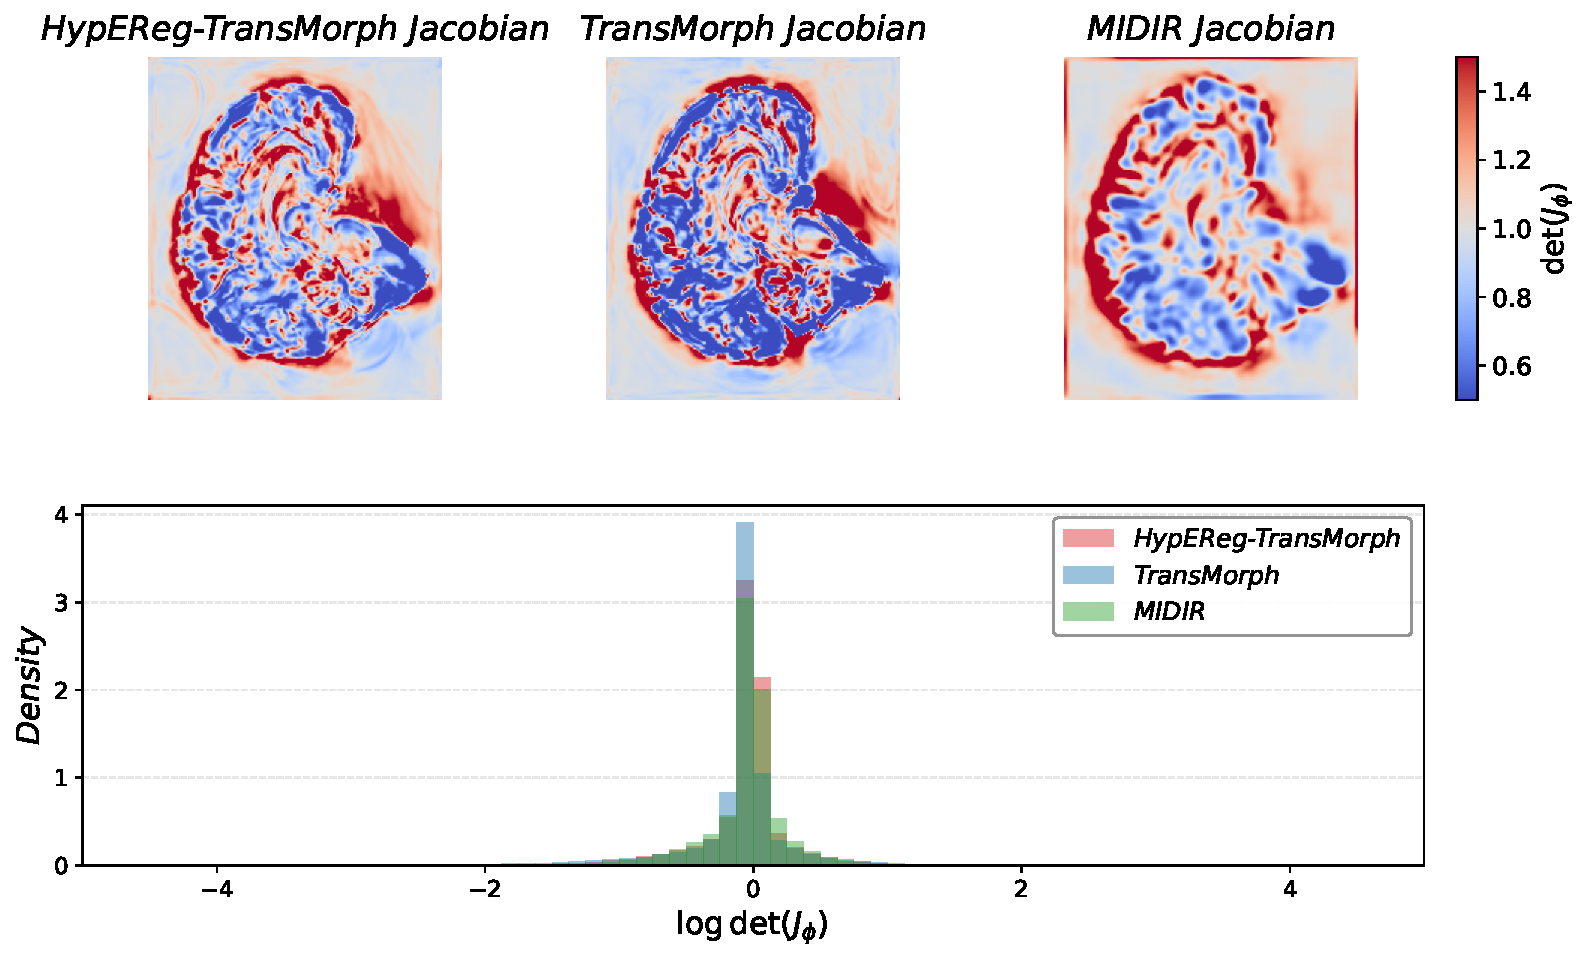
\includegraphics[width=0.96\textwidth]{figures/fig4_jacobian.pdf}
\caption{Jacobian-determinant analysis for deformation plausibility. Top-row heatmaps show spatial maps of \(\det(J_\phi)\) on a central slice for each model, where values near 1 indicate near-volume-preserving local transforms and extreme values indicate expansion/compression. The bottom histogram reports \(\log(\det(J_\phi))\) over voxels; narrower distributions centered near zero indicate more stable local volume behavior. This figure supports the folding-suppression behavior of HypEReg-TransMorph. (HER-TransMorph in figure panels denotes HypEReg-TransMorph.)\label{fig4}}
\end{figure}

For models with subject-level per-case exports, inferential results support these trends: HypEReg-TransMorph significantly improves regularity relative to TransMorph on non-positive Jacobian ratio and SDlogJ after FDR correction (both \(q<0.001\)); compared with MIDIR, HypEReg-TransMorph shows a significant disadvantage on SDlogJ and non-positive Jacobian ratio (both \(q<0.001\)), while HD95 difference is not significant (\(q=0.592\)); compared with SyN, HypEReg-TransMorph shows significantly lower HD95 (\(q<0.001\)) but higher SDlogJ (\(q<0.001\)). Using the newly uploaded TransMorph and TransMorphBayes checkpoints, an additional paired analysis on Dice and non-positive Jacobian ratio confirms HypEReg-TransMorph advantages versus both uploaded baselines after FDR correction (Supplementary Table~S2).

\subsection{Efficiency}
To resolve the inference-cost discrepancy, we re-profiled pure forward inference under an isolated protocol that excludes metric computation and label warping. Under this protocol, HypEReg-TransMorph and TransMorph show nearly identical forward cost (0.4316 s vs.\ 0.4306 s on a representative IXI case) and peak memory (5.422 GB vs.\ 5.421 GB), consistent with identical inference architecture/parameter count (46.771 M). Larger end-to-end timing differences in previous tables are therefore attributable to evaluation-path operations rather than mandatory model-forward overhead.

\subsection{Qualitative Visualization}
Representative qualitative registration/deformation visualizations are shown in Figures~\ref{fig2} and~\ref{fig3}. In this representative case, HypEReg-TransMorph qualitatively suggests improved boundary alignment near selected ventricular/cortical regions, while preserving smooth deformation grids and reducing visible fold-prone patterns. These visual observations complement the quantitative metrics in Table~\ref{tab2}.

\noindent A descriptive multi-metric overview (Dice, non-positive Jacobian ratio, SDlogJ, and HD95) is provided as Figure~S1 in the Supplementary Materials.

\begin{table}[H]
\caption{Main IXI model comparison (115-subject protocol).\label{tab2}}
\centering
\scriptsize
\setlength{\tabcolsep}{3pt}
\begin{tabularx}{\textwidth}{lccccc}
\toprule
\textbf{Model} & \textbf{Dice\(\uparrow\)} & \(\boldsymbol{\det(J_\phi)\le 0}\) \textbf{ratio \(\downarrow\)} & \textbf{SDlogJ\(\downarrow\)} & \textbf{HD95 (mm)\(\downarrow\)} & \textbf{ASSD (mm)\(\downarrow\)}\\
\midrule
HypEReg-TransMorph & \textbf{0.7537 \(\pm\) 0.0275} & 0.000015 \(\pm\) 0.000007 & 0.3280 \(\pm\) 0.0221 & \textbf{3.1561 \(\pm\) 0.5408} & \textbf{0.5891 \(\pm\) 0.1021}\\
TransMorph & 0.7527 \(\pm\) 0.0305 & 0.015021 \(\pm\) 0.003416 & 0.5064 \(\pm\) 0.0250 & 5.8794 \(\pm\) 0.8048 & 1.5593 \(\pm\) 0.2416\\
TransMorphBayes & \underline{0.7530 \(\pm\) 0.0302} & 0.015634 \(\pm\) 0.003363 & 0.4920 \(\pm\) 0.0330 & \underline{3.3745 \(\pm\) 0.6740} & \underline{0.6215 \(\pm\) 0.1305}\\
VoxelMorph-1 & 0.7293 \(\pm\) 0.0290 & 0.015860 \(\pm\) 0.003388 & 0.4999 \(\pm\) 0.0327 & 5.7156 \(\pm\) 0.8168 & 1.4696 \(\pm\) 0.1962\\
CycleMorph & 0.7366 \(\pm\) 0.0303 & 0.017192 \(\pm\) 0.003819 & 0.5176 \(\pm\) 0.0320 & 5.7789 \(\pm\) 0.8317 & 1.4638 \(\pm\) 0.2038\\
MIDIR & 0.7423 \(\pm\) 0.0228 & \textbf{0.000000 \(\pm\) 0.000000} & \underline{0.3148 \(\pm\) 0.0242} & 5.3028 \(\pm\) 0.6139 & 1.4100 \(\pm\) 0.1585\\
CoTr & 0.7347 \(\pm\) 0.0290 & 0.012975 \(\pm\) 0.003430 & 0.4874 \(\pm\) 0.0331 & 5.5691 \(\pm\) 0.7931 & 1.4278 \(\pm\) 0.1828\\
nnFormer & 0.7472 \(\pm\) 0.0294 & 0.015946 \(\pm\) 0.003584 & 0.5167 \(\pm\) 0.0371 & 5.8274 \(\pm\) 0.8195 & 1.4322 \(\pm\) 0.1878\\
PVT & 0.7273 \(\pm\) 0.0330 & 0.018578 \(\pm\) 0.003141 & 0.5431 \(\pm\) 0.0318 & 5.9286 \(\pm\) 0.8264 & 1.5253 \(\pm\) 0.2069\\
SyN (ANTs) & 0.6445 \(\pm\) 0.0397 & \underline{0.000001 \(\pm\) 0.000005} & \textbf{0.2996 \(\pm\) 0.0725} & 6.4457 \(\pm\) 1.8104 & 1.5233 \(\pm\) 0.7748\\
\bottomrule
\end{tabularx}
\parbox{\textwidth}{\footnotesize Values are reported as mean \(\pm\) standard deviation over 115 test subjects. Dice and \(\det(J_\phi)\le 0\) ratio are computed from per-case evaluation tables; SDlogJ/HD95/ASSD are taken from the same finalized IXI summary exports used for manuscript tabulation. Bold indicates best value per metric; underline indicates second-best.}
\end{table}


\begin{table}[H]
\caption{End-to-end evaluation-path efficiency comparison (runtime, peak memory, and parameter count) for selected baselines.\label{tab3}}
\begin{tabularx}{\textwidth}{lccc}
\toprule
\textbf{Model} & \textbf{Runtime (s/case)\(\downarrow\)} & \textbf{Peak Memory (GB)\(\downarrow\)} & \textbf{Parameters (M)}\\
\midrule
HypEReg-TransMorph & 0.2034 & 10.635 & 46.771 \\
TransMorphBayes & 3.5372 & 16.088 & 46.771 \\
TransMorph & 0.0953 & 5.601 & 46.771 \\
VoxelMorph-1 & 0.0359 & 5.162 & 0.274 \\
CycleMorph & 0.0501 & 5.085 & 0.361 \\
MIDIR & 0.0203 & 5.085 & 0.266 \\
CoTr & 0.1127 & 5.307 & 38.738 \\
nnFormer & 0.0675 & 5.336 & 45.328 \\
SyN (ANTs) & N/A & N/A & N/A \\
\bottomrule
\end{tabularx}
\noindent{\footnotesize{These values are from the end-to-end evaluation path, which includes model forward, label warping, and metric computation. Isolated pure-forward profiling for HypEReg-TransMorph and TransMorph is discussed in Section~4.3; measured no-gradient forward runtime and peak memory are reported in the Supplementary Materials (\textit{Supplementary Experimental Details} / \textit{Model and Environment Configuration}). Peak memory for deep models is computed from per-case runtime records. Parameter counts are computed from loaded model weights/checkpoints. For classical methods (SyN), learned-parameter count is not applicable. SyN is a classical iterative optimizer; its runtime and peak memory are not directly comparable to feed-forward learned models and vary with subject anatomy and CPU configuration.}}
\end{table}

\begin{figure}[t]
\centering
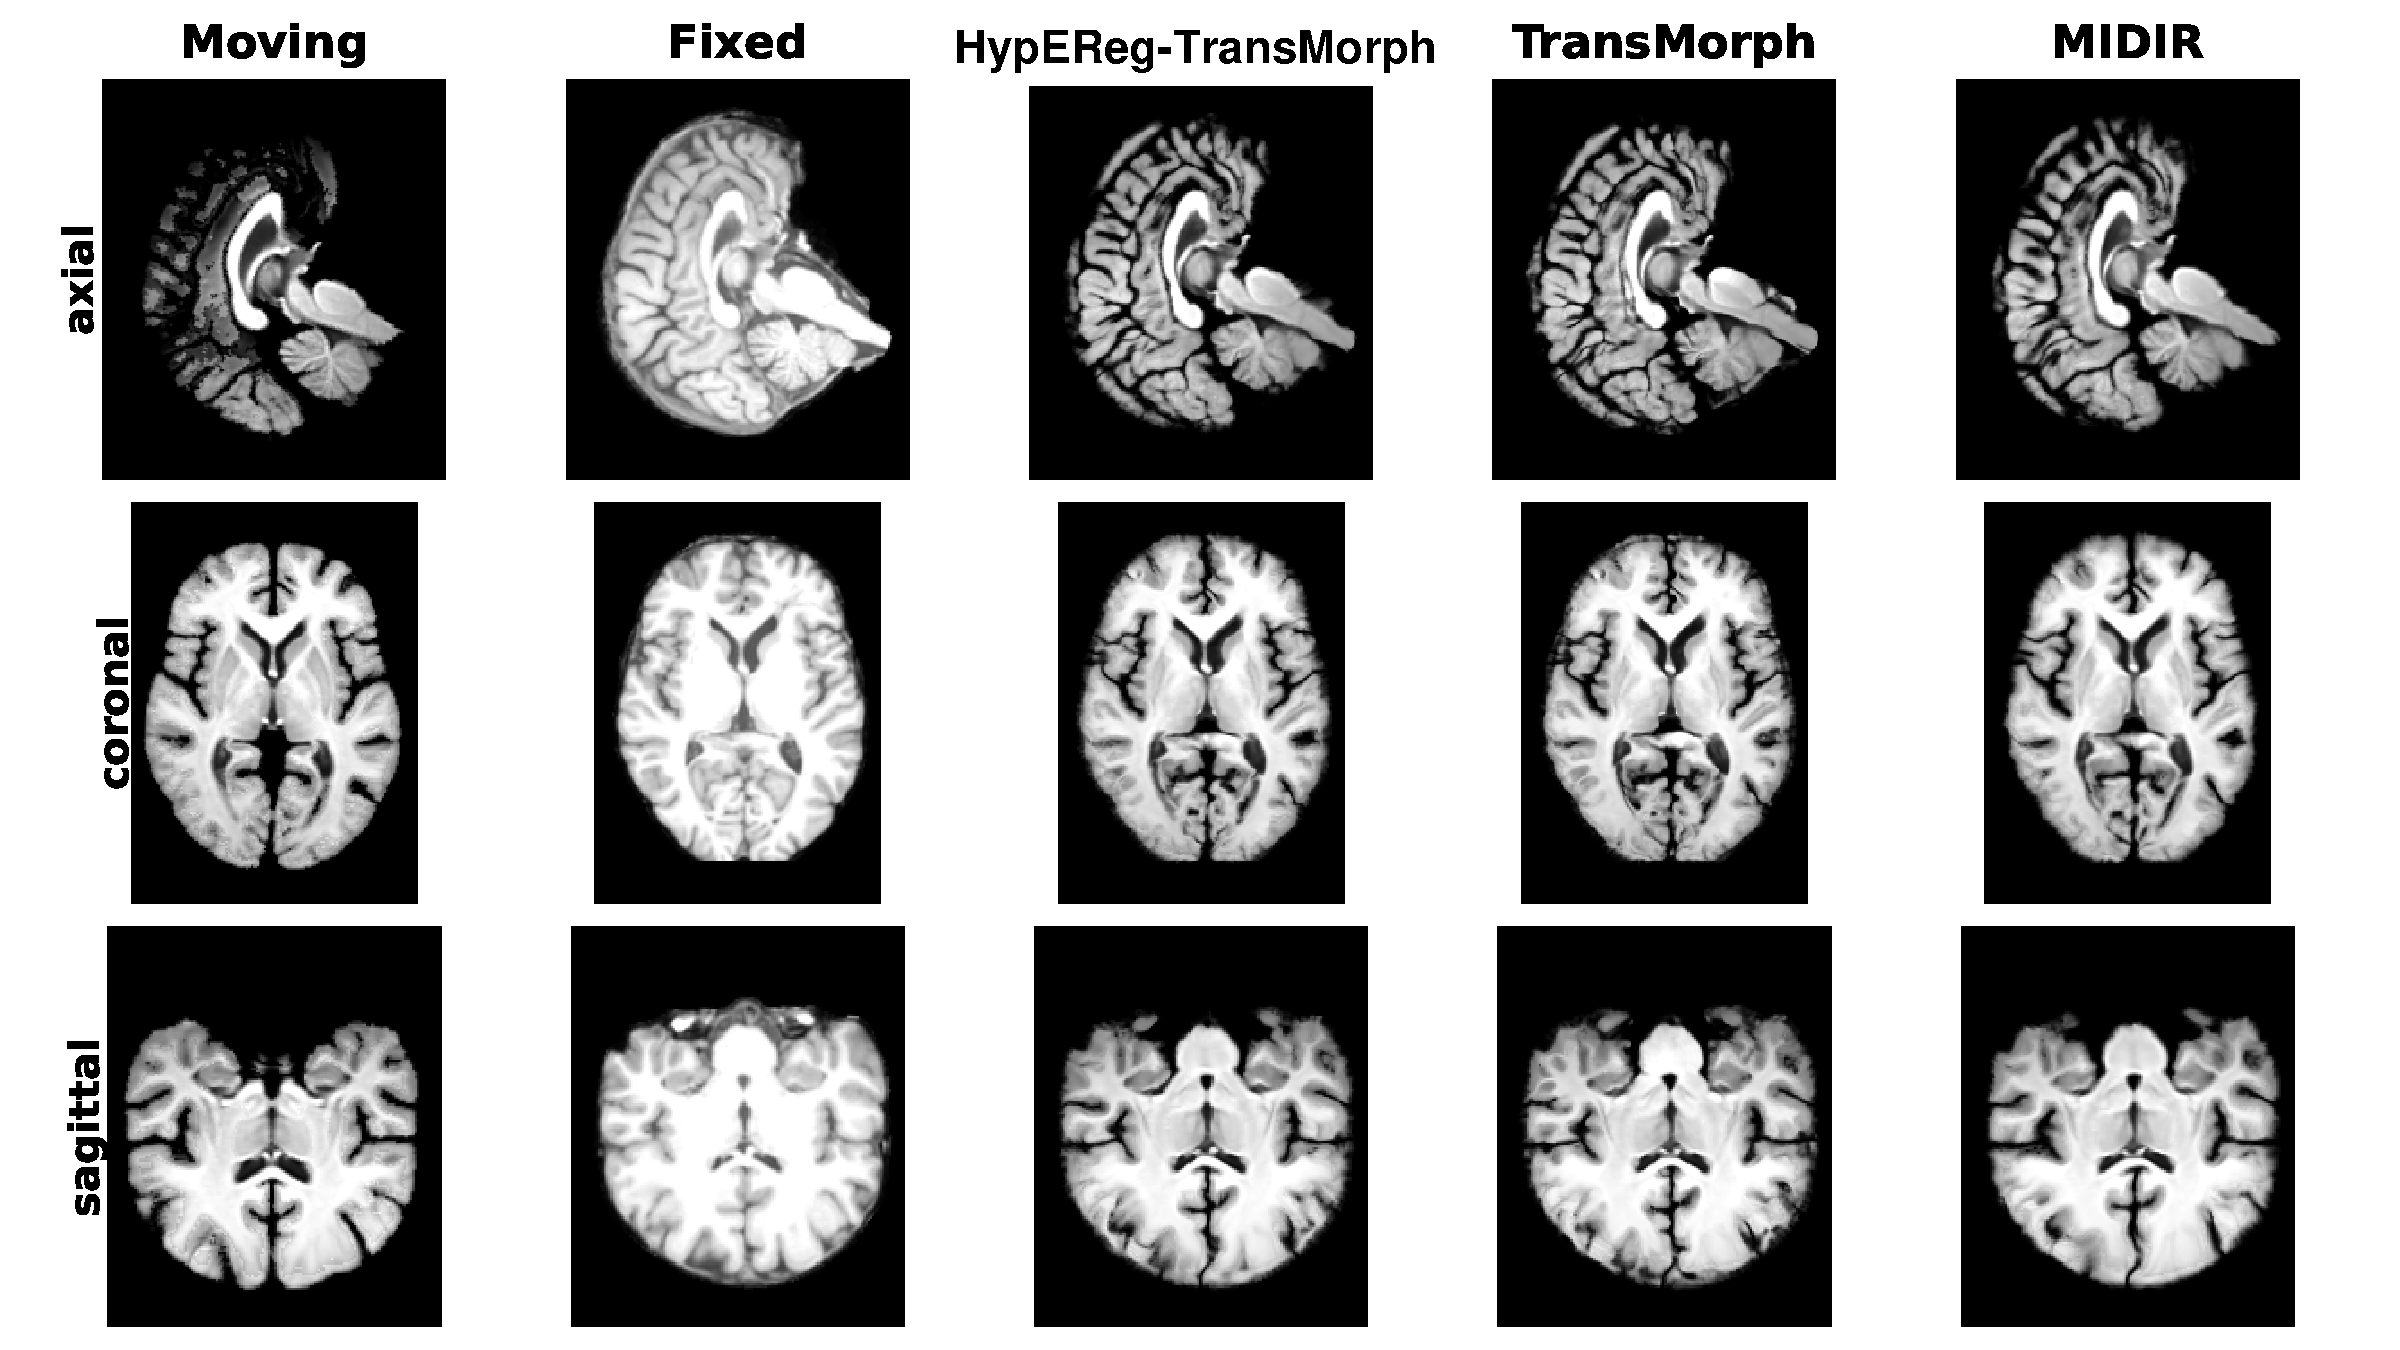
\includegraphics[width=0.96\textwidth]{figures/fig2_qualitative.pdf}
\caption{Qualitative registration comparison on a representative IXI test subject across three orthogonal views (axial/coronal/sagittal). Columns show moving atlas, fixed target, and warped outputs from HypEReg-TransMorph, TransMorph, and MIDIR. Figure~\ref{fig2} qualitatively highlights boundary-alignment behavior in ventricles, cortex, and deep gray structures, complementing the quantitative trends reported in the Results section. (HER-TransMorph in figure panels denotes HypEReg-TransMorph.) \label{fig2}}
\end{figure}

\begin{figure}[t]
\centering
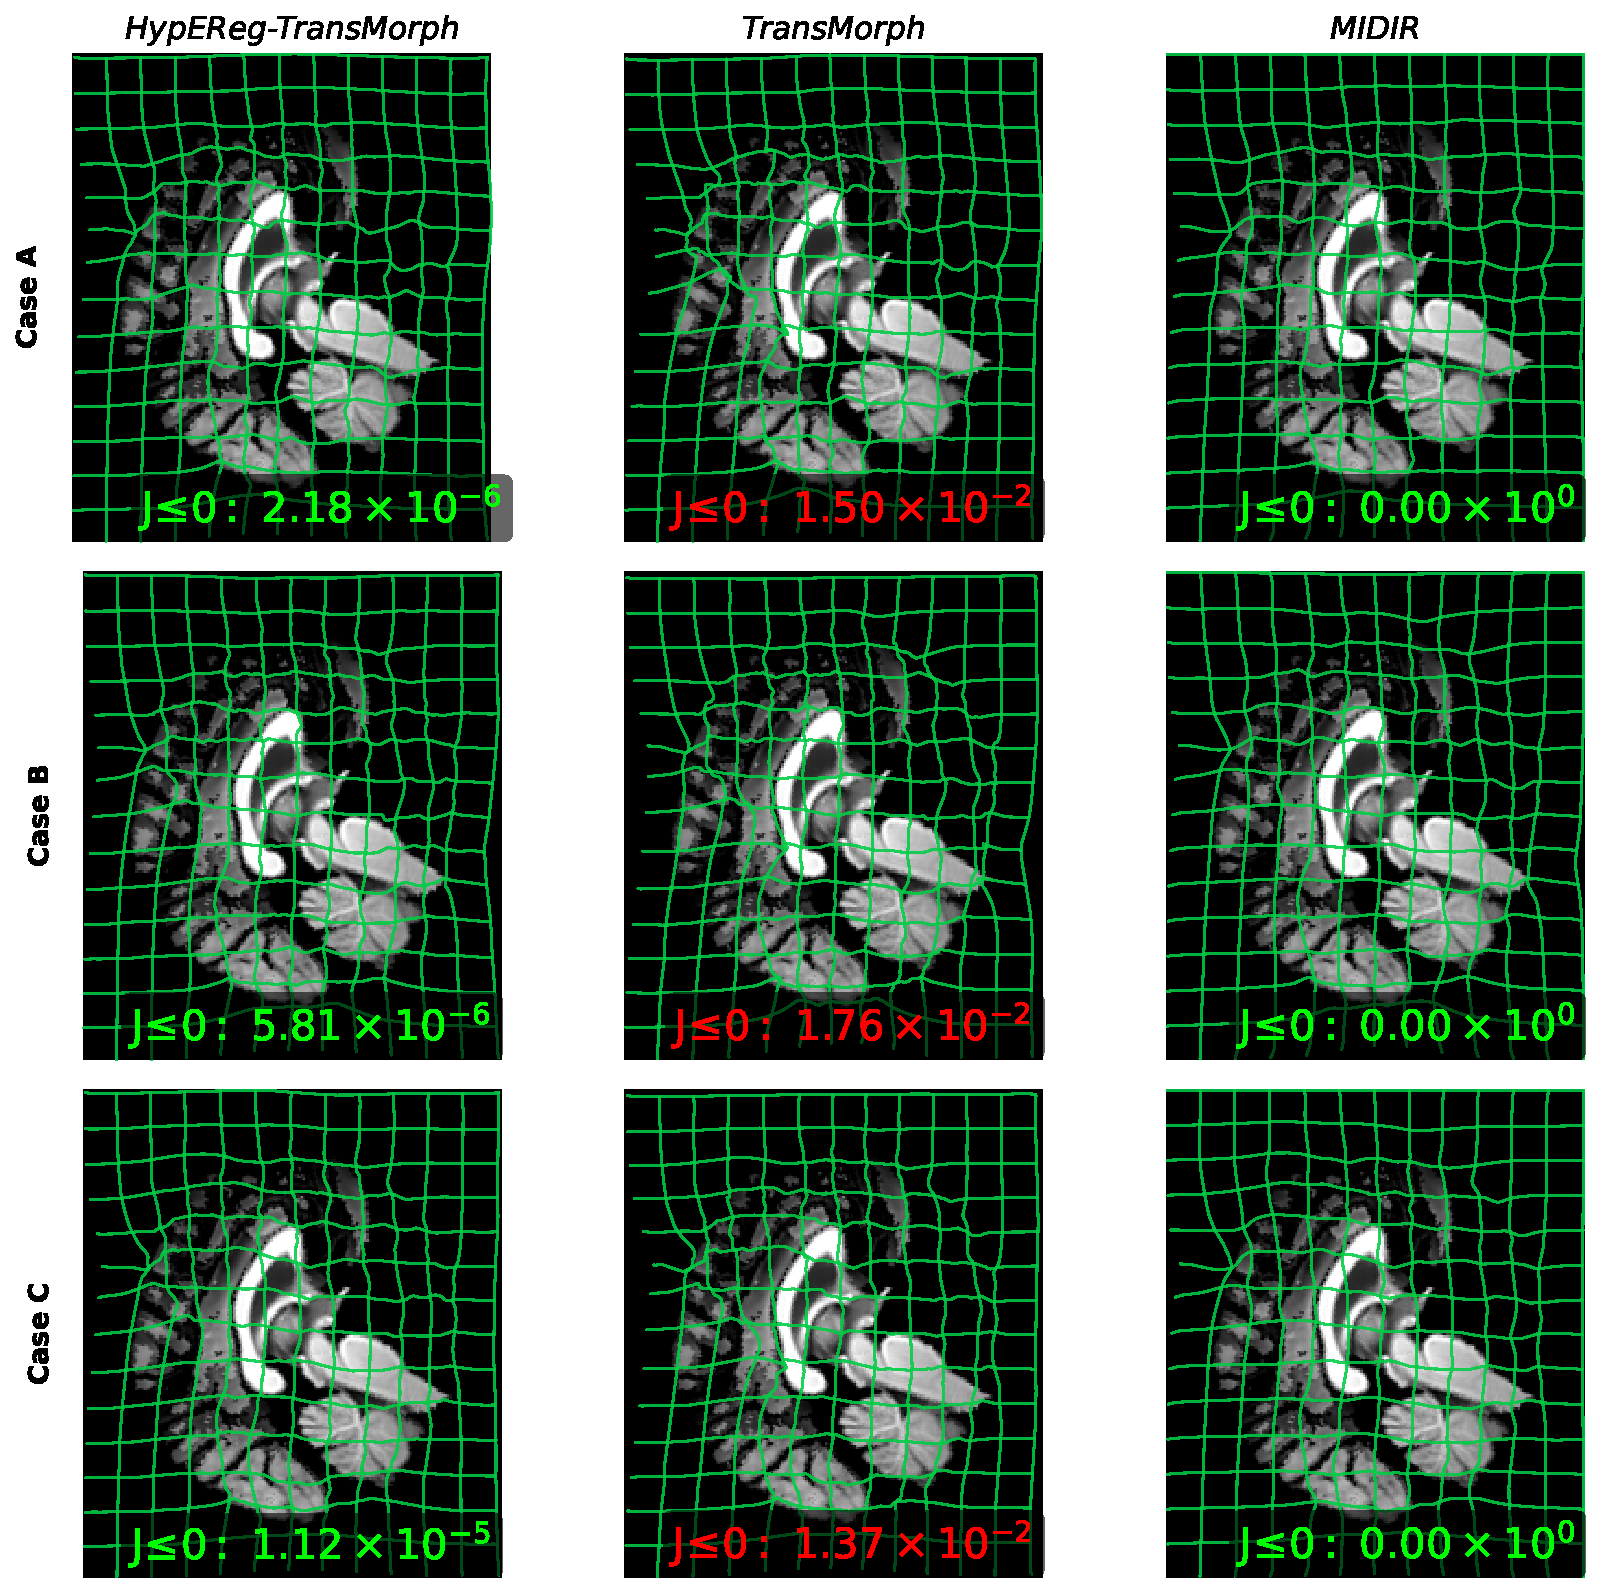
\includegraphics[width=0.96\textwidth]{figures/fig3_gridwarp.pdf}
\caption{Deformation-grid visualization derived from predicted displacement fields on the same IXI subject. Cyan lattice lines represent transformed coordinates after warping by each model. Smooth, non-self-intersecting grids indicate stable local geometry, whereas abrupt kinks or crossings indicate folding risk. In this representative case, HypEReg-TransMorph qualitatively suggests smoother global transitions and fewer folding-prone patterns. (HER-TransMorph in figure panels denotes HypEReg-TransMorph.)\label{fig3}}
\end{figure}

% Figure S1 note moved to ?4.4 above.

% Figure 5 moved to supplementary discussion to keep the main text focused on
% metrics with direct inferential/statistical support in final submission.

%%%%%%%%%%%%%%%%%%%%%%%%%%%%%%%%%%%%%%%%%%
\section{Discussion}

This work is positioned as a deformation-quality improvement study rather than a pure overlap-accuracy competition. The key result is that HypEReg-TransMorph improves Jacobian regularity and folding suppression (lower non-positive Jacobian determinant ratio and SDlogJ) while maintaining comparable Dice/HD95/ASSD to strong Transformer baselines. This trade-off is practically meaningful for downstream morphometric tasks that are sensitive to local folding artifacts.

The observed performance pattern suggests that adding physically motivated regularization to Transformer-based registration can constrain unrealistic local volume changes without substantially degrading alignment fidelity. In clinical and research workflows, this is relevant for Jacobian-based analyses, longitudinal disease progression studies, and atlas-based quantification where deformation plausibility matters beyond overlap scores.

The CNN/B-spline baseline MIDIR also achieves zero non-positive Jacobian ratio on IXI, with SDlogJ (0.3148) marginally lower than HypEReg-TransMorph (0.3280). The two methods reach comparable regularity through different routes: MIDIR enforces smoothness implicitly via B-spline parameterization, while HypEReg-TransMorph enforces regularity explicitly through differentiable Jacobian penalties on dense flow. HypEReg acts as a drop-in regularizer for dense-displacement backbones without changing inference parameterization, and preserves overlap expressivity (Dice 0.7537 vs.\ 0.7423 for MIDIR on IXI).

Conceptually, HypEReg differs from inverse-consistency focused regularizers (e.g., ICON~\cite{greer2021icon}/GradICON~\cite{tian2023gradicon}) and hierarchical deformation constructions (e.g., LapIRN~\cite{mok2020lapirn}): HypEReg directly penalizes local Jacobian volume distortion and folding in the objective, whereas inverse-consistency methods target cycle/inverse agreement and Laplacian-pyramid formulations target multi-scale deformation composition. These constraints are complementary rather than mutually exclusive.

\noindent\textbf{Positioning relative to elastic and hyperelastic regularization in deep registration.}
Our work is best understood as one configuration in a broader research line that injects elastic or hyperelastic regularization into learned registration. The selective Jacobian-determinant penalty of \citet{mok2020fast} is the conceptual antecedent of $\mathcal{L}_{\mathrm{fold}}$ in CNN-based diffeomorphic registration; the BMR-style volume-change penalty plus curvature regularizer of \citet{hering2021lung} demonstrates that BMR-flavored Jacobian control can be embedded in CNN lung-CT registration loss; \citet{zou2023conformal} use a non-linear, conformal-invariant hyperelastic energy in a deep registration framework on lung CT; and the \emph{ElasticMorph} framework~\cite{elasticmorph2025} plugs a second-order Navier--Cauchy linear-elastic regularizer into TransMorph and VoxelMorph backbones and reports overlap improvements with reduced folding artifacts on IXI/LPBA40. Relative to these, our contribution is intentionally narrow in scope: (i) we use a non-linear volume-distortion penalty plus an explicit hinge rather than linear elasticity, which targets local volumetric implausibility directly through $\det J_\phi$ rather than through divergence/curl operators; (ii) we evaluate the Transformer-backbone instantiation on the IXI atlas-to-subject protocol with paired Wilcoxon/BH-FDR inferential statistics on subject-level metrics; and (iii) we do not claim originality for the hyperelastic principle or the anti-folding penalty themselves, which derive from BMR \cite{burger2013hyperelastic} and from \citet{mok2020fast}, respectively. A direct head-to-head comparison with ElasticMorph on a shared IXI evaluation is left to future work, as that framework reports its results under a different protocol and was not retrained in this manuscript.

\noindent\textbf{Clinical and translational significance.}
The improvements reported here translate into several concrete benefits for medical imaging practice. (i) \emph{Trustworthy morphometric biomarkers.} Lower SDlogJ and a near-zero non-positive Jacobian ratio mean that voxel-wise log-Jacobian maps---used as surrogates of regional atrophy/expansion in tensor-based morphometry---are no longer corrupted by spurious negative-determinant voxels, so longitudinal volume-change estimates around the hippocampus, ventricles and cortical mantle reflect genuine biological change rather than registration artefacts. This is directly relevant to imaging endpoints in Alzheimer's disease, mild cognitive impairment, multiple sclerosis and other progressive disorders, where small effect sizes are routinely overwhelmed by registration noise. (ii) \emph{Atlas-based segmentation and treatment planning.} A fold-free warp guarantees that label propagation from atlas to subject is one-to-one, which is the assumption required by atlas-fusion segmentation pipelines used for FreeSurfer-style cortical parcellation, radiotherapy organ-at-risk delineation, and pre-surgical planning of deep-brain-stimulation or epilepsy resection targets; the lower bending energy and near-zero \(\det J_\phi \le 0\) ratio reduce the manual-correction burden on clinical readers. (iii) \emph{Image-guided intervention and population studies.} Combined with the maintained Dice/HD95/ASSD performance and the very small forward latency reported in Section~4.3 (\(\sim\)0.43~s per volume on a single GPU), HypEReg-TransMorph supports both intra-operative use cases (where smooth, invertible deformations are required for accurate landmark warping) and large-scale population studies (where thousands of subjects must be processed without manual quality-control flagging of folded fields). (iv) \emph{Drop-in upgrade path for existing clinical research pipelines.} Because HypEReg modifies only the loss function and leaves the inference architecture and parameter count unchanged (Table~\ref{tab3}), existing TransMorph-based workflows in academic and hospital research groups can adopt it without retraining downstream tools or reconfiguring deployment infrastructure. Together, these properties target the central usability gap in current learning-based brain-MRI registration: high overlap accuracy is no longer obtained at the cost of physically implausible deformations, which we view as a prerequisite for translating learned registration from benchmark tables into reproducible clinical neuroimaging analysis.

Future work will extend HypEReg-TransMorph to multi-modal registration, pathology-rich cohorts, and uncertainty-aware registration frameworks. Another direction is adaptive hyperelastic weighting to better balance local accuracy and topology constraints under heterogeneous anatomical deformations. Beyond methodological extensions, prospective clinical validation on disease-specific cohorts (e.g., ADNI for Alzheimer's progression, OASIS for ageing, BraTS for tumour-bearing brains) will be needed to quantify how the observed regularity gains translate into improved sensitivity of derived biomarkers and reduced reader workload in real reporting workflows.

%%%%%%%%%%%%%%%%%%%%%%%%%%%%%%%%%%%%%%%%%%
\section{Conclusions}

HypEReg-TransMorph introduces a hyperelastic-subset regularizer (volume + anti-folding at \(\alpha=0\)) into a TransMorph-style deformable registration framework and reduces local folding relative to unconstrained dense Transformer baselines while maintaining statistically indistinguishable grouped-VOI Dice. Under the IXI atlas-to-subject protocol, HypEReg improves the non-positive Jacobian determinant ratio and SDlogJ relative to TransMorph and TransMorphBayes, although MIDIR and SyN remain strong on selected regularity metrics. These results support HypEReg as a useful dense-flow regularization strategy and motivate further multi-seed, cross-dataset, and downstream morphometric validation.

From a clinical neuroimaging perspective, the gain in deformation regularity directly addresses a long-standing usability barrier of learning-based registration: Jacobian-based biomarkers, atlas-fusion segmentations, and longitudinal morphometry pipelines all assume one-to-one, fold-free warps, an assumption that unconstrained Transformer backbones routinely violate. By delivering near-diffeomorphic fields at feed-forward inference speed and with no change to the deployment architecture, HypEReg-TransMorph offers a drop-in upgrade path for brain-MRI research and clinical-research pipelines---ranging from atrophy quantification in neurodegenerative disease to atlas-based delineation for radiotherapy and surgical planning---without sacrificing the throughput and reproducibility advantages that motivated the move from classical iterative methods to learned registration in the first place. This positions Jacobian-aware regularization as a practical, low-cost step toward clinically deployable Transformer-based deformable registration.

%%%%%%%%%%%%%%%%%%%%%%%%%%%%%%%%%%%%%%%%%%
\vspace{6pt} 

%%%%%%%%%%%%%%%%%%%%%%%%%%%%%%%%%%%%%%%%%%
%% optional
\supplementary{Supplementary Materials (separate PDF) include: Table~S1 (inferential summary for selected baselines), Table~S2 (paired inferential statistics with Wilcoxon+BH-FDR), Table~S3 (grouped-VOI label mapping), Figure~S1 (descriptive IXI multi-metric overview), implementation and profiling details, and additional qualitative registration/Jacobian visualizations.}

% Only for journal Methods and Protocols:
% If you wish to submit a video article, please do so with any other supplementary material.
% \supplementary{The following supporting information can be downloaded at: \linksupplementary{s1}, Figure S1: title; Table S1: title; Video S1: title. A supporting video article is available at doi: link.}

% Only used for preprtints:
% \supplementary{The following supporting information can be downloaded at the website of this paper posted on \href{https://www.preprints.org/}{Preprints.org}.}

% Only for journal Hardware:
% If you wish to submit a video article, please do so with any other supplementary material.
% \supplementary{The following supporting information can be downloaded at: \linksupplementary{s1}, Figure S1: title; Table S1: title; Video S1: title.\vspace{6pt}\\
%\begin{tabularx}{\textwidth}{lll}
%\toprule
%\textbf{Name} & \textbf{Type} & \textbf{Description} \\
%\midrule
%S1 & Python script (.py) & Script of python source code used in XX \\
%S2 & Text (.txt) & Script of modelling code used to make Figure X \\
%S3 & Text (.txt) & Raw data from experiment X \\
%S4 & Video (.mp4) & Video demonstrating the hardware in use \\
%... & ... & ... \\
%\bottomrule
%\end{tabularx}
%}

%%%%%%%%%%%%%%%%%%%%%%%%%%%%%%%%%%%%%%%%%%
\authorcontributions{Conceptualization, S.X. and M.X.; methodology, S.X. and M.X.; software, S.X.; validation, S.X. and M.X.; formal analysis, S.X.; investigation, S.X.; data curation, S.X.; writing---original draft preparation, S.X.; writing---review and editing, S.X. and M.X.; visualization, S.X.; supervision, M.X.; project administration, M.X. All authors have read and agreed to the published version of the manuscript.}

\funding{This research received no external funding.}

\institutionalreview{Not applicable. This study performed secondary analysis of publicly available anonymized IXI data and did not recruit new human participants.}

\informedconsent{Not applicable to this secondary-analysis study using publicly available anonymized data.}

\dataavailability{Source code, configuration files, per-case metric tables, and figure/statistics scripts are openly available at \url{https://github.com/Zzxmh/HypEReg-TransMorph} and archived at Zenodo: \url{https://doi.org/10.5281/zenodo.19888526} \cite{xu2026hypereg_zenodo}. Trained model weights are available from the corresponding author upon reasonable request. The IXI dataset used in this study is publicly available at \url{https://brain-development.org/ixi-dataset/} (CC BY-SA 3.0). The preprocessed split follows the public TransMorph-style IXI preprocessing release.}

%\durcstatement{Current research is limited to the [please insert a specific academic field, e.g., XXX], which is beneficial [share benefits and/or primary use] and does not pose a threat to public health or national security. Authors acknowledge the dual-use potential of the research involving xxx and confirm that all necessary precautions have been taken to prevent potential misuse. As an ethical responsibility, authors strictly adhere to relevant national and international laws about DURC. Authors advocate for responsible deployment, ethical considerations, regulatory compliance, and transparent reporting to mitigate misuse risks and foster beneficial outcomes.}

% Only for journal Nursing Reports
%\publicinvolvement{Please describe how the public (patients, consumers, carers) were involved in the research. Consider reporting against the GRIPP2 (Guidance for Reporting Involvement of Patients and the Public) checklist. If the public were not involved in any aspect of the research add: ``No public involvement in any aspect of this research''.}
%
%% Only for journal Nursing Reports
%\guidelinesstandards{Please add a statement indicating which reporting guideline was used when drafting the report. For example, ``This manuscript was drafted against the XXX (the full name of reporting guidelines and citation) for XXX (type of research) research''. A complete list of reporting guidelines can be accessed via the equator network: \url{https://www.equator-network.org/}.}
%
%% Only for journal Nursing Reports
%\useofartificialintelligence{Please describe in detail any and all uses of artificial intelligence (AI) or AI-assisted tools used in the preparation of the manuscript. This may include, but is not limited to, language translation, language editing and grammar, or generating text. Alternatively, please state that ?AI or AI-assisted tools were not used in drafting any aspect of this manuscript?.}

\acknowledgments{The authors thank the maintainers of open-source registration baselines and the IXI data contributors.}

\conflictsofinterest{The authors declare no conflicts of interest.}

%%%%%%%%%%%%%%%%%%%%%%%%%%%%%%%%%%%%%%%%%%
%% Optional

%% Only for journal Encyclopedia
%\entrylink{The Link to this entry published on the encyclopedia platform.}

\abbreviations{Abbreviations}{
The following abbreviations are used in this manuscript:
\\
\noindent
\begin{tabular}{@{}ll}
HypEReg & Hyperelastic-Energy Regularization\\
MRI & Magnetic Resonance Imaging\\
HD95 & 95th percentile Hausdorff Distance\\
ASSD & Average Symmetric Surface Distance\\
NCC & Normalized Cross-Correlation\\
LNCC & Local Normalized Cross-Correlation\\
SDlogJ & Standard Deviation of Log Jacobian Determinant\\
IXI & Information eXtraction from Images dataset\\
BMR & Burger--Modersitzki--Ruthotto (hyperelastic energy framework)\\
FDR & False Discovery Rate
\end{tabular}
}

%%%%%%%%%%%%%%%%%%%%%%%%%%%%%%%%%%%%%%%%%%
%\isPreprints{}{% This command is only used for ``preprints''.
\begin{adjustwidth}{-\extralength}{0cm}
%} % If the paper is ``preprints'', please uncomment this parenthesis.
%\printendnotes[custom] % Un-comment to print a list of endnotes

\reftitle{References}

% Please provide either the correct journal abbreviation (e.g. according to the ?List of Title Word Abbreviations? http://www.issn.org/services/online-services/access-to-the-ltwa/) or the full name of the journal.
% Citations and References in Supplementary files are permitted provided that they also appear in the reference list here. 

%=====================================
% References, variant A: external bibliography
%=====================================
\bibliography{refs}

%=====================================
% References, variant B: internal bibliography
%=====================================
\iffalse

% ACS format
\isAPAandChicago{}{%
\begin{thebibliography}{999}
% Reference 1
\bibitem[Author1(year)]{ref-journal}
Author~1, T. The title of the cited article. {\em Journal Abbreviation} {\bf 2008}, {\em 10}, 142--149.
% Reference 2
\bibitem[Author2(year)]{ref-book1}
Author~2, L. The title of the cited contribution. In {\em The Book Title}; Editor 1, F., Editor 2, A., Eds.; Publishing House: City, Country, 2007; pp. 32--58.
% Reference 3
\bibitem[Author1 and Author2 (year)]{ref-book2}
Author 1, A.; Author 2, B. \textit{Book Title}, 3rd ed.; Publisher: Publisher Location, Country, 2008; pp. 154--196.
% Reference 4
\bibitem[Author4(year)]{ref-unpublish}
Author 1, A.B.; Author 2, C. Title of Unpublished Work. \textit{Abbreviated Journal Name} year, \textit{phrase indicating stage of publication (submitted; accepted; in press)}.
% Reference 5
\bibitem[Author8(year)]{ref-url}
Title of Site. Available online: URL (accessed on Day Month Year).
% Reference 6
\bibitem[Author6(year)]{ref-proceeding}
Author 1, A.B.; Author 2, C.D.; Author 3, E.F. Title of presentation. In Proceedings of the Name of the Conference, Location of Conference, Country, Date of Conference (Day Month Year); Abstract Number (optional), Pagination (optional).
% Reference 7
\bibitem[Author7(year)]{ref-thesis}
Author 1, A.B. Title of Thesis. Level of Thesis, Degree-Granting University, Location of University, Date of Completion.
\end{thebibliography}
}

% Chicago format (Used for journal: arts, genealogy, histories, humanities, jintelligence, laws, literature, religions, risks, socsci)
\isChicagoStyle{%
\begin{thebibliography}{999}
% Reference 1
\bibitem[Aranceta-Bartrina(1999a)]{ref-journal}
Aranceta-Bartrina, Javier. 1999a. Title of the cited article. \textit{Journal Title} 6: 100--10.
% Reference 2
\bibitem[Aranceta-Bartrina(1999b)]{ref-book1}
Aranceta-Bartrina, Javier. 1999b. Title of the chapter. In \textit{Book Title}, 2nd ed. Edited by Editor 1 and Editor 2. Publication place: Publisher, vol. 3, pp. 54?96.
% Reference 3
\bibitem[Baranwal and Munteanu {[1921]}(1955)]{ref-book2}
Baranwal, Ajay K., and Costea Munteanu. 1955. \textit{Book Title}. Publication place: Publisher, pp. 154--96. First published 1921 (op-tional).
% Reference 4
\bibitem[Berry and Smith(1999)]{ref-thesis}
Berry, Evan, and Amy M. Smith. 1999. Title of Thesis. Level of Thesis, Degree-Granting University, City, Country. Identifi-cation information (if available).
% Reference 5
\bibitem[Cojocaru et al.(1999)]{ref-unpublish}
Cojocaru, Ludmila, Dragos Constatin Sanda, and Eun Kyeong Yun. 1999. Title of Unpublished Work. \textit{Journal Title}, phrase indicating stage of publication.
% Reference 6
\bibitem[Driver et al.(2000)]{ref-proceeding}
Driver, John P., Steffen Rohrs, and Sean Meighoo. 2000. Title of Presentation. In \textit{Title of the Collected Work} (if available). Paper presented at Name of the Conference, Location of Conference, Date of Conference.
% Reference 7
\bibitem[Harwood(2008)]{ref-url}
Harwood, John. 2008. Title of the cited article. Available online: URL (accessed on Day Month Year).
\end{thebibliography}
}{}

% APA format (Used for journal: admsci, behavsci, businesses, econometrics, economies, education, ejihpe, games, humans, ijfs, journalmedia, jrfm, languages, psycholint, publications, tourismhosp, youth)
\isAPAStyle{%
\begin{thebibliography}{999}
% Reference 1
\bibitem[\protect\citeauthoryear{Azikiwe \BBA\ Bello}{{2020a}}]{ref-journal}
Azikiwe, H., \& Bello, A. (2020a). Title of the cited article. \textit{Journal Title}, \textit{Volume}(Issue), 
Firstpage--Lastpage/Article Number.
% Reference 2
\bibitem[\protect\citeauthoryear{Azikiwe \BBA\ Bello}{{2020b}}]{ref-book1}
Azikiwe, H., \& Bello, A. (2020b). \textit{Book title}. Publisher Name.
% Reference 3
\bibitem[Davison(1623/2019)]{ref-book2}
Davison, T. E. (2019). Title of the book chapter. In A. A. Editor (Ed.), \textit{Title of the book: Subtitle} 
(pp. Firstpage--Lastpage). Publisher Name. (Original work published 1623) (Optional).
% Reference 4
\bibitem[Fistek et al.(2017)]{ref-proceeding}
Fistek, A., Jester, E., \& Sonnenberg, K. (2017, Month Day). Title of contribution [Type of contribution]. Conference Name, Conference City, Conference Country.
% Reference 5
\bibitem[Hutcheson(2012)]{ref-thesis}
Hutcheson, V. H. (2012). \textit{Title of the thesis} [XX Thesis, Name of Institution Awarding the Degree].
% Reference 6
\bibitem[Lippincott \& Poindexter(2019)]{ref-unpublish}
Lippincott, T., \& Poindexter, E. K. (2019). \textit{Title of the unpublished manuscript} [Unpublished manuscript/Manuscript in prepara-tion/Manuscript submitted for publication]. Department Name, Institution Name.
% Reference 7
\bibitem[Harwood(2008)]{ref-url}
Harwood, J. (2008). \textit{Title of the cited article}. Available online: URL (accessed on Day Month Year).
\end{thebibliography}
}{}
\fi

% If authors have biography, please use the format below
%\section*{Short Biography of Authors}
%\bio
%{\raisebox{-0.35cm}{\includegraphics[width=3.5cm,height=5.3cm,clip,keepaspectratio]{Definitions/author1.pdf}}}
%{\textbf{Firstname Lastname} Biography of first author}
%
%\bio
%{\raisebox{-0.35cm}{\includegraphics[width=3.5cm,height=5.3cm,clip,keepaspectratio]{Definitions/author2.jpg}}}
%{\textbf{Firstname Lastname} Biography of second author}

% For the MDPI journals use author-date citation, please follow the formatting guidelines on http://www.mdpi.com/authors/references
% To cite two works by the same author: \citeauthor{ref-journal-1a} (\citeyear{ref-journal-1a}, \citeyear{ref-journal-1b}). This produces: Whittaker (1967, 1975)
% To cite two works by the same author with specific pages: \citeauthor{ref-journal-3a} (\citeyear{ref-journal-3a}, p. 328; \citeyear{ref-journal-3b}, p.475). This produces: Wong (1999, p. 328; 2000, p. 475)

%%%%%%%%%%%%%%%%%%%%%%%%%%%%%%%%%%%%%%%%%%
%% for journal Sci
%\reviewreports{\\
%Reviewer 1 comments and authors? response\\
%Reviewer 2 comments and authors? response\\
%Reviewer 3 comments and authors? response
%}
%%%%%%%%%%%%%%%%%%%%%%%%%%%%%%%%%%%%%%%%%%
\PublishersNote{}
%\isPreprints{}{% This command is only used for ``preprints''.
\end{adjustwidth}
%} % If the paper is ``preprints'', please uncomment this parenthesis.
\end{document}

